%----------------------------------------------------------------------------------------
% Preambulo y Configuración
%----------------------------------------------------------------------------------------

\documentclass[
    11pt,
    spanish,
    singlespacing,
    parskip,
    headsepline,
    bookmarks=true,
    unicode=true,
    pdftoolbar=true,
    pdfmenubar=true,
    pdffitwindow=false,
    colorlinks=true,
    linkcolor=blue,
    citecolor=blue,
    urlcolor=blue
]{MastersDoctoralThesis}

\usepackage[utf8]{inputenc} % Codificación de entrada UTF-8
\usepackage[T1]{fontenc}    % Codificación de salida para caracteres especiales
\usepackage{graphicx}       % Manejo de gráficos
\usepackage{eso-pic}        % Permite agregar fondos
\usepackage{hyperref}       % Manejo de hipervínculos y marcadores

% Redefinición de caracteres problemáticos en marcadores
\hypersetup{
    pdftitle={Título del Documento},
    pdfauthor={Autor del Documento},
    pdfkeywords={Sistemas Embebidos, Internet de las Cosas, Inteligencia Artificial},
    pdfstartview={FitH},
    unicode=true,
    colorlinks=true,
    linkcolor=blue,
    citecolor=blue,
    urlcolor=blue
}

\pdfstringdefDisableCommands{%
  \def\texttt#1{#1}%
  \def\textbf#1{#1}%
  \def\textit#1{#1}%
  \def\"{\"}%
  \def\~{~}%
  \def\'{'}%
  \def\^{}%
  \def\textunderscore{\_} % Manejo del subrayado en marcadores
}


% Definir comandos requeridos por la clase
\newcommand{\degreename}{Maestría en Ciencias} % Cambia según tu título
\newcommand{\univname}{Universidad Nacional de Ejemplo} % Cambia según tu universidad
\newcommand{\keywordnames}{Palabras clave:}
%----------------------------------------------------------------------------------------
% Documento Principal
%----------------------------------------------------------------------------------------

\begin{document}

% Configuración de la portada
\posgrado{Carrera / Maestría}
\keywords{Sistemas Embebidos, Internet de las Cosas, Inteligencia Artificial}

% Incluir la portada desde un archivo separado
\include{portada}

% Configuración del contenido preliminar
\frontmatter % Usar numeración romana para las páginas preliminares
\pagestyle{plain} % Estilo de encabezado simple

%----------------------------------------------------------------------------------------
% Resumen
%----------------------------------------------------------------------------------------

\begin{abstract}
\addchaptertocentry{\abstractname} % Agregar resumen al índice
En esta memoria se describe el análisis, diseño y puesta en marcha de un sistema que permite detectar si una empresa puede entrar en quiebra.
Este sistema será ofrecido como un servicio con el fin de proporcionar información estratégica a potenciales clientes. De esta manera clientes como analistas de riegos, ejecutivos de créditos, entre otros, podrán tomar decisiones críticas en sus negocios.

La resolución de este trabajo fue posible gracias a la implementación de conocimientos aprendidos durante la especialización, tales como técnicas de análisis de datos, modelos de machine learning, automatización de procesos en entornos de mlops y puesta en producción de modelos mediante APIs.
\end{abstract}

%----------------------------------------------------------------------------------------
% Agradecimientos
%----------------------------------------------------------------------------------------

\begin{acknowledgements}
\vspace{1.5cm}
Esta sección es para agradecimientos personales y es totalmente \textbf{OPCIONAL}.
\end{acknowledgements}

%----------------------------------------------------------------------------------------
% Índice
%----------------------------------------------------------------------------------------

\tableofcontents
\listoffigures
\listoftables

%----------------------------------------------------------------------------------------
% Dedicatoria
%----------------------------------------------------------------------------------------

\dedicatory{\textbf{Dedicado a... [OPCIONAL]}}

%----------------------------------------------------------------------------------------
% Capítulos
%----------------------------------------------------------------------------------------

\mainmatter % Iniciar numeración numérica para el contenido principal
\pagestyle{thesis} % Estilo de encabezado de tesis

% Incluir capítulos desde archivos separados
% Chapter 1

\chapter{Introducción general} % Main chapter title

\label{Chapter1} % For referencing the chapter elsewhere, use \ref{Chapter1} 
\label{IntroGeneral}

En este capítulo se explica la importancia de la predicción de quiebra de empresas. Luego, se detalla el estado del arte actual respecto a esta temática. Se explican también las motivaciones detrás de este trabajo. Finalmente, se describen los objetivos y alcance del trabajo.

%----------------------------------------------------------------------------------------

% Define some commands to keep the formatting separated from the content 
\newcommand{\keyword}[1]{\textbf{#1}}
\newcommand{\tabhead}[1]{\textbf{#1}}
\newcommand{\code}[1]{\texttt{#1}}
\newcommand{\file}[1]{\texttt{\bfseries#1}}
\newcommand{\option}[1]{\texttt{\itshape#1}}
\newcommand{\grados}{$^{\circ}$}

%----------------------------------------------------------------------------------------

%\section{Introducción}

%----------------------------------------------------------------------------------------
\section{Predicción de quiebra de empresas}

Predecir si una empresa entra en quiebra es información de gran valor para distintos actores del mercado financiero. Acceder a esta información en tiempo y forma le permitirá a bancos, compañías aseguradoras, fondos de inversión o consultoras especializadas en riesgo crediticio tomar mejores decisiones en sus respectivas labores.

El presente trabajo es un emprendimiento personal orientado a la resolución de la problemática presentada. Para llevarlo a cabo, se utiliza el dataset de \textit{Taiwanese Bankruptcy Prediction}\citep{taiwanese_bankruptcy_prediction_572}, el cual contiene información financiera de empresas del mercado de Taiwán entre 1999 y 2009, y fue publicado por el \textit{Taiwan Economic Journal}\footnote{\url{https://www.tejwin.com/en/}}. Esta información será utilizada en el entorno de trabajo que se puede apreciar en la figura \ref{fig:diagBloques}. En este, se refina la información, se entrenan distintos modelos de machine learning, y se comparan dichos modelos a fin de elegir al mejor de ellos. Los resultados obtenidos se publican mediante un servicio web, para que los distintos interesados pueden consultarlos y utilizarlos según sus necesidades.

\begin{figure}[htbp]
	\centering
	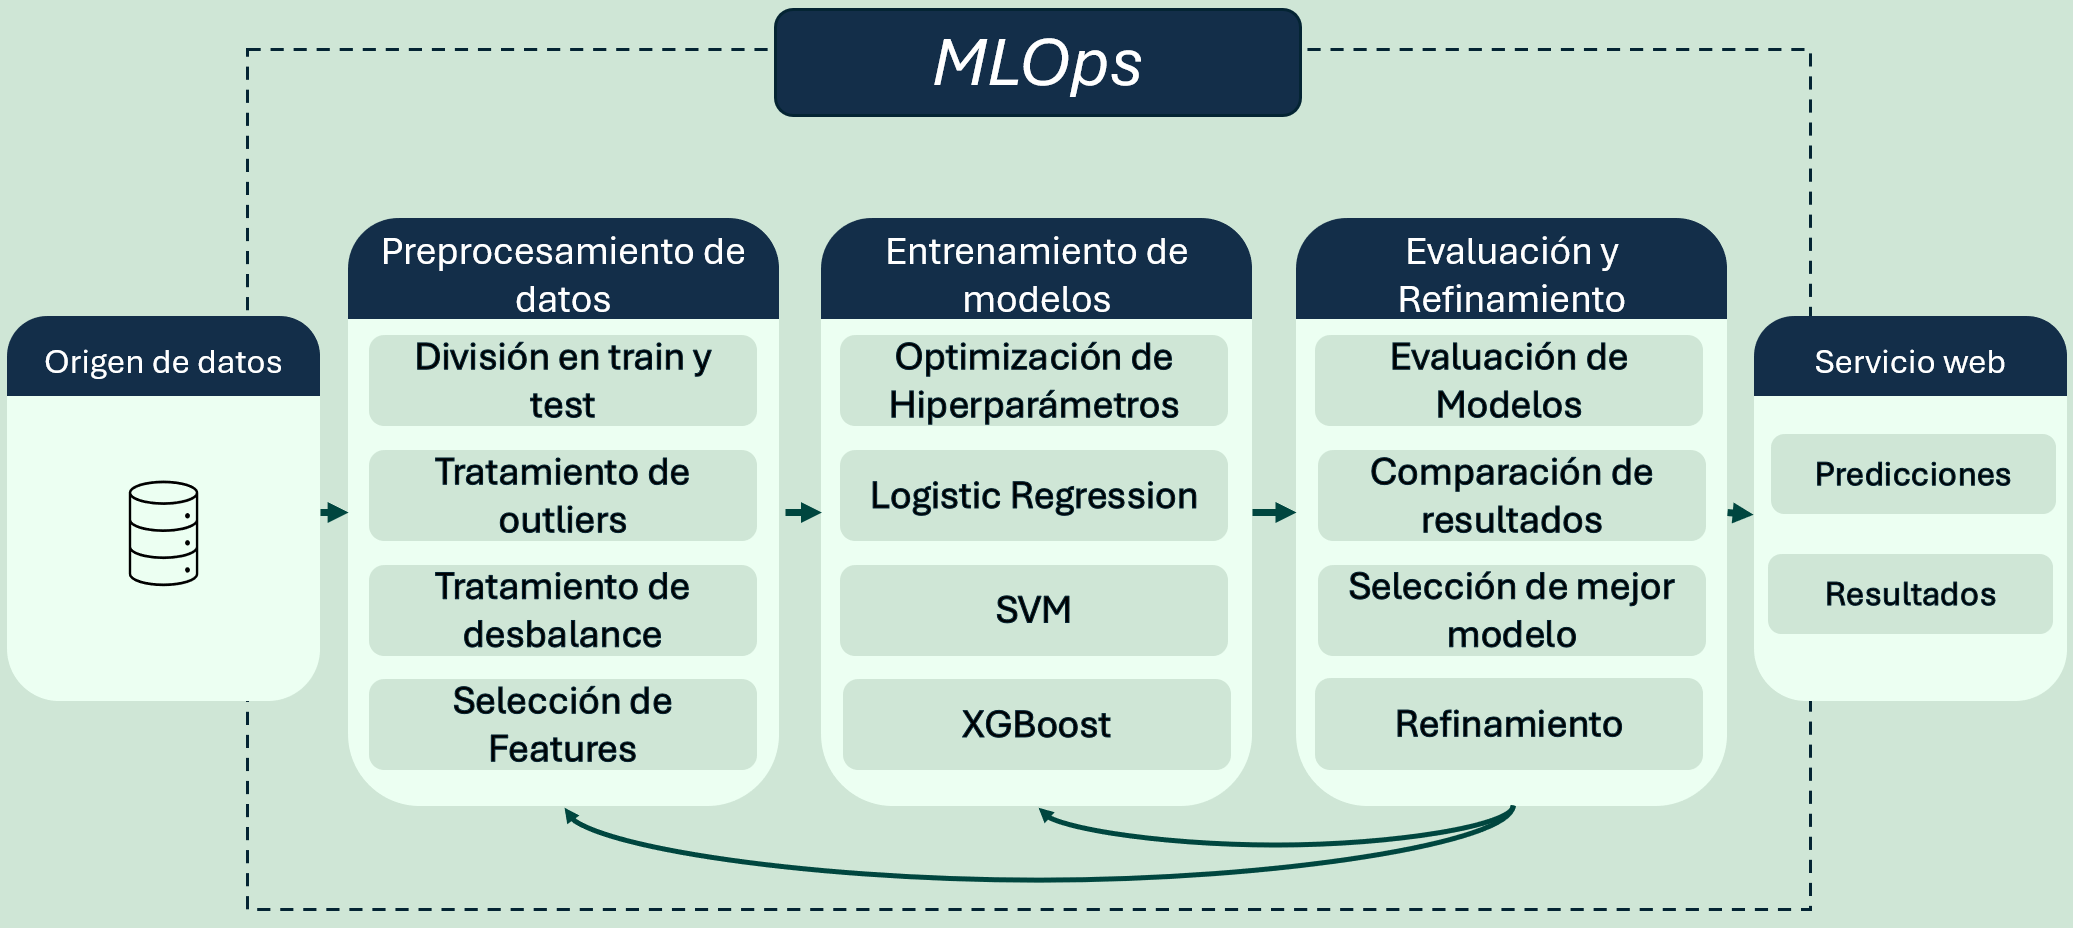
\includegraphics[width=\textwidth]{Figures/diagramaEnBloques.png}
	\caption{Diagrama en bloques.}
	\label{fig:diagBloques}
\end{figure}

%----------------------------------------------------------------------------------------

\section{Estado del arte}

Existen diversos estudios basados en el dataset de \textit{Taiwanese Bankruptcy Prediction}\citep{taiwanese_bankruptcy_prediction_572}. En algunos de ellos, como en \textit{Comprehensive Evaluation of Bankruptcy Prediction in Taiwanese Firms Using Multiple Machine Learning Models}, se exploran modelos de \textit{machine learning} tales como SVM (\textit{Support Vector Machine})\citep{model:svm} y \textit{Random Forest}\citep{model:rf}. En otros, se analiza cómo ciertas técnicas afectan a las predicciones finales. Por ejemplo, en \textit{Undersampling bankruptcy prediction: Taiwan bankruptcy data}\citep{10.1371/journal.pone.0254030} se estudian los resultados de aplicar técnicas de preprocesamiento de datos mediante \textit{undersampling}.

Independientemente de los modelos y de las técnicas de preprocesamiento utilizadas, los estudios actuales se limitan a presentar resultados numéricos y conclusiones sobre las herramientas utilizadas, pero ninguno permite utilizar los modelos obtenidos para realizar predicciones reales.

%----------------------------------------------------------------------------------------

\section{Motivación}

Este trabajo busca solucionar las siguientes problemáticas:

\begin{itemize}
\item Permitir a actores del mercado financiero predecir si una empresa entra en quiebra.
\item Resolver las limitaciones de trabajos actuales, en donde solo se presentan resultados numéricos y conclusiones.
\end{itemize}

Por ello, se diseña y desarrolla un sistema que implementa técnicas y modelos de \textit{machine learning}. Estos modelos, son entrenados, refinados y comparados para encontrar al que mejor prediga si una empresa entra en quiebra. Una vez seleccionado el mejor de ellos, se lo expone mediante un servicio web, a fin de que distintos interesados puedan utilizarlo según sus necesidades.

%----------------------------------------------------------------------------------------

\section{Objetivos y alcance}

Este trabajo busca crear y exponer, mediante servicio web, un sistema que prediga si una empresa entra en quiebra.
Para ello, se define un entorno de trabajo que se caracteriza por ser iterativo, reproducible y escalable, en donde se usa un dataset de origen público\citep{taiwanese_bankruptcy_prediction_572}. Sobre este dataset se aplicarán técnicas de preprocesamiento de datos para mejorarlo. Luego, se entrenarán modelos de \textit{machine learning}, que permitan realizar las predicciones deseadas. Estos modelos serán evaluados y comparados entre sí, a fin de encontrar al "mejor" de ellos. El mejor modelo y los resultados obtenidos serán expuestos mediante un servicio web, para que cualquier interesado pueda hacer uso de ellos. Sobre estos resultados se vuelven a aplicar las técnicas ya mencionadas, para poder refinarlos y reevaluarlos.

A partir de esto, se define el siguiente alcance:

\begin{itemize}
\item Análisis exploratorio de datos: se estudia al dataset en cuestión, para poder conocer mejor sus características, distribuciones, y potenciales errores a corregir.
\item Preprocesamiento de datos: se aplican técnicas para eliminar duplicados, corrección de datos faltantes, corrección de \textit{outliers}, balanceo de datos, entre otras.
\item Implementación de modelos de \textit{machine learning}: se implementan modelos como SVM\citep{model:svm}, \textit{logistic regression}\citep{model:lr} y \textit{XGBoost}\citep{model:xgboost}.
\item Evaluación de modelos: se obtienen métricas y gráficos asociados a cada modelo, para poder compararlos entre sí.
\item Automatización: se automatizan los pasos anteriores, a fin de preparar los resultados para el servicio web.
\item Trackeo de resultados: se utiliza el servicio \textit{MLFlow}\citep{WEBSITE:mlflow} para hacer seguimiento de los modelos entrenados y sus métricas.
\item Creación de un servicio web: se crea una \textit{API} web la cual expone al mejor modelo entrenado, como así también las métricas y gráficos de todos los modelos.
\end{itemize}

De la misma manera, se definen las actividades que quedan excluídas de este trabajo:

\begin{itemize}
\item Despliegue del servicio en plataformas de \textit{cloud computing}, tales como Azure\citep{WEBSITE:azure}, AWS\citep{WEBSITE:aws}, Google Cloud\citep{WEBSITE:gcp}, entre otras.
\item Creación de interfaz web: el trabajo se limita hasta la creación de una \textit{API} web, la cual se podrá utilizar mediante herramientas existentes, tales como \textit{cURL}\citep{WEBSITE:curl} y otras similares.
\item Comercialización y distribución: el trabajo se limita a la creación del sistema descrito, más no a su comercialización y/o distribución.
\end{itemize}
\chapter{Introducción específica} % Main chapter title

\label{Chapter2}

En este capítulo se comienza detallando las técnicas de procesamiento de datos utilizadas en el trabajo.
Luego, se describen los modelos de \textit{machine learning} entrenados.
Posteriormente, se describen las distintas herramientas utilizadas para hacer seguimiento de modelos, para automatizar el procesamiento de datos y entrenamiento de modelos, como así también de aquellas empleadas en el desarrollo de APIs y contenedores.

%----------------------------------------------------------------------------------------
\section{Técnicas de procesamiento de datos}
\label{subsec:tecnicas_procesamiento}

En este trabajo se emplearon distintas técnicas de procesamiento de datos, que permitieron detectar y tratar \textit{outliers}, escalar variables, balancear el dataset y seleccionar features. En la tabla \ref{tab:procesamiento} se presentan las técnicas utilizadas.

\begin{table}[h]
	\centering
	\caption[Técnicas utilizadas]{Técnicas utilizadas en el procesamiento de datos.}
	\begin{tabular}{c l}
		\toprule
		\textbf{Técnica} 	 & \textbf{Utilizada para}\\
		\midrule
        IQR \citep{article:iqr}                                             & Detección de \textit{outliers} \\
		Imputación por media \citep{article:mean_median_imputation}         & Tratamiento de \textit{outliers} \\
        Imputación por mediana \citep{article:mean_median_imputation}       & Tratamiento de \textit{outliers} \\
        Imputación por moda \citep{article:mode_imputation}                 & Tratamiento de \textit{outliers} \\
        Imputación por raíz cuadrada \citep{article:sqrt_transformation}    & Tratamiento de \textit{outliers} \\
        Imputación de Yeo-Johnson \citep{article:yeojohnson}                & Tratamiento de \textit{outliers} \\
        \textit{Standard scaler} \citep{WEBSITE:standardscaler}             & Escalado de variables \\
        SMOTE \citep{article:smote}                         & Balanceo de dataset \\
        SMOTE-ENN \citep{article:smoteenn}                  & Balanceo de dataset \\
        ADASYN \citep{article:adasyn}                       & Balanceo de dataset \\
        Información mutua \citep{article:mutualinformation} & Selección de features \\
		\bottomrule
		\hline
	\end{tabular}
	\label{tab:procesamiento}
\end{table}

\subsection{Detección y tratamiento de outliers}

En este tipo de trabajo, en el que se entrenan modelos de modelos de \textit{machine learning}, suelen utilizarse datasets con una gran cantidad de variables (columnas) y datos (registros).

Las variables de estos datasets suelen presentar distintos tipos de distribuciones matemáticas, que deben ser analizadas a fin de descubrir sus características. Entre estas se encuentran los valores atípicos u \textit{outliers}, cuya presencia no solo afecta a la propia distribución, sino también al rendimiento de los modelos.

Por este motivo, uno de los procesamientos que se implementan en este trabajo es el de detectar y tratar \textit{outliers}.

Para detectarlos, se utiliza la técnica de IQR o rango intercuartil \citep{article:iqr}. Esta mide la dispersión del 50\% central de los datos, es decir, aquellos que se encuentran entre el percentil 25 (cuartil 1 o Q1) y el percentil 75 (cuartil 3 o Q3), y se define mediante la ecuación \ref{eq:iqr}.

\begin{equation}
	\label{eq:iqr}
	IQR = Q3 - Q1
\end{equation}

Una vez definido el rango intercuartil, se consideran \textit{outliers} a aquellos valores que se encuentran 1,5 veces el IQR debajo del cuartil 1, o 1,5 veces el IQR sobre el cuartil 3, tal como se define en la ecuación \ref{eq:outlier}.

\begin{equation}
    \label{eq:outlier}
    outlier(x) = 
\begin{cases}
    \text{No es outlier} & Q_1 - 1,5*IQR \le x \le Q_3 + 1,5*IQR \\
    \text{Sí es outlier} &  \text{para todo otro caso }
\end{cases}
\end{equation}

Una vez detectados los \textit{outliers}, se imputan mediante distintas técnicas, entre las que se encuentran:

\begin{itemize}
\item Imputación por media: reemplaza los valores atípicos con el valor medio de la distribución.
\item Imputación por mediana: reemplaza los valores atípicos con la mediana de la distribución.
\item Imputación por moda: reemplaza los valores atípicos con la moda de la distribución.
\item Transformación por raíz cuadrada: aplica la función de raíz cuadrada sobre la columna entera.
\item Transformación de Yeo-Johnson \citep{article:yeojohnson}: permite normalizar datos, estabilizar la varianza y reducir el sesgo en una distribución. Es una mejora de la transformación Box-Cox \citep{article:boxcox}, ya que funciona con cualquier número real.
\end{itemize}

\subsection{Escalado de variables}

Además de los \textit{outliers}, las magnitudes de las variables de un dataset pueden también afectar el rendimiento de los modelos. Por ejemplo, si una variable tiene un rango de valores entre 0 y 100 y otra entre 0 y 1000, el modelo puede interpretar que la segunda es más importante, lo cual podría ser erróneo.

Para solucionar estos inconvenientes se utilizan técnicas de escalado de variables.

En particular, se utiliza la técnica de \textit{Standard Scaler} \citep{WEBSITE:standardscaler}, cuya fórmula se observa en la ecuación \ref{eq:standardscaler}. Esta transforma los datos de una variable para que tengan una media ($\mu$) de 0 y una desviación estándar ($\sigma$) de 1, es decir, asemeja la distribución a la de una normal.

\begin{equation}
	\label{eq:standardscaler}
	z = \frac{x-\mu}{\sigma}
\end{equation}

\subsection{Balanceo de dataset}
\label{subsec:tecnicas_balanceo}

Al trabajar con problemas de clasificación, los datasets implementados tienen una columna \textit{target} u objetivo, la cual describe a una clase a la cual pertenece cada registro. Una de las particularidades que se pueden presentar es la del desbalance: una clase tiene una cantidad mucho mayor de casos que el resto. Estas se conocen como clases dominantes, y su presencia puede afectar el rendimiento de modelos de \textit{machine learning} al hacer que estos ignoren a las clases minoritarias.

Para solucionar este problema, se utilizan técnicas de sobremuestreo u \textit{oversampling}, las cuales agregan registros extras al dataset con el fin de tener un dataset balanceado.

En este trabajo se utilizan las siguientes técnicas:
\begin{itemize}
    \item SMOTE \citep{article:smote}: permite generar ejemplos sintéticos en función de un caso de la clase minoritaria y sus vecinos más cercanos.
    \item ADASYN \citep{article:adasyn}: consiste en una evolución de SMOTE, la cual genera datos sintéticos en áreas donde la densidad de la clase minoritaria es baja y está rodeada de la clase mayoritaria.
    \item SMOTE-ENN \citep{article:smoteenn}: consiste en una técnicas que comienza aplicando SMOTE, para luego eliminar ejemplos de clases que difieran de sus vecinos mediante ENN (\textit{Edited Nearest Neighbors}).
\end{itemize}

\subsection{Selección de features}
\label{subsec:seleccion_features}

Otra particularidad de los datasets utilizados en este tipo de trabajo es la cantidad de variables presentes. Estos valores suelen ser muy variados, ya que hay datasets con menos de 10 variables (como el iris dataset \citep{WEBSITE:iris-dataset}, que tiene 6 columnas), mientras que otros pueden tener 100 y más columnas.

Para estos últimos casos resulta conveniente aplicar técnicas de selección de características o \textit{features}. Estas nos permiten filtrar algunas columnas con el fin de quedarse con las más importantes. De esta manera, se elimina cierto ruido de datos pocos relevantes, como así también se reduce el sobreajuste (u \textit{overfitting}) al entrenar modelos.

En particular, en este trabajo se hace uso de la técnica de información mutua o \textit{mutual information} \citep{article:mutualinformation}. Esta permite permite cuantificar cuánta información se obtiene sobre la variable objetivo al utilizar una característica en particular, es decir, que tan dependientes son entre sí. A mayor valor, mayor es la información que una \textit{feature} nos proporciona sobre la variable objetivo. Por eso, se busca obtener la información mutua de todas las columnas frente al \textit{target}, luego se hace un ranking ordenando de mayor a menor, y finalmente se selecciona un subconjunto de las mejores variables de dicho ranking.

%----------------------------------------------------------------------------------------
\section{Modelos de inteligencia artificial}

En los trabajos de clasificación mediante datasets, los primeros pasos y tareas suelen dedicarse a la preparación del dataset, utilizando técnicas como las mencionadas anteriormente. Una vez preparado, los datasets son utilizados como entrada de distintos algoritmos de \textit{machine learning} con el fin de obtener un modelo. Estos modelos posteriormente nos permiten realizar predicciones o clasificaciones a partir de datos particulares de entrada.

En este trabajo, se implementan los siguientes modelos de \textit{machine learning}:

\begin{itemize}
    \item Regresión logística o \textit{logistic regression} \citep{model:lr}: permite obtener la probabilidad de pertenencia a una de las clases de estudio. A partir de dicha probabilidad se determina a qué clase pertenece una muestra en particular.
    \item SVM o \textit{support vector machine} \citep{model:svm}: se caracteriza por buscar un hiperplano que separe las clases de estudio con el margen más amplio posible.
    \item XGBoost \citep{model:xgboost}: consiste en un modelo de ensambles basado en árboles de decisión. Estos árboles son entrenados de manera secuencial, especializándose en corregir los errores del árbol anterior. Esto permite que sea un modelo robusto al evitar el sobreajuste.
\end{itemize}

%----------------------------------------------------------------------------------------
\section{Optimización de hiperparámetros}

Los modelos de \textit{machine learning} se caracterizan por tener hiperparámetros: variables de configuración que se definen antes de comenzar el entrenamiento. Estas se diferencian de un parámetro ya que controlan como se comporta el algoritmo.

A partir de esto, surge la necesidad de optimizar estos hiperparámetros con el fin de encontrar un equilibrio óptimo entre sesgo y varianza, lo cual a su vez permite evitar el sobreajuste (\textit{overfitting}) o subajuste (\textit{underfitting} del modelo.

En este trabajo se utiliza el \textit{framework} optuna \citep{WEBSITE:optuna}: una biblioteca de código abierto basada en python. Esta utiliza una optimización bayesiana para, en lugar de probar valores al azar, aprender de intentos anteriores y enfocarse en las combinaciones de hiperparámetros más prometedoras, encontrando así las más óptimas.

%----------------------------------------------------------------------------------------
\section{Herramientas - Tracking server}

Al trabajar con distintos modelos de \textit{machine learning} resulta crucial hacer un seguimiento de los mismos, enfocándose en los datos o datasets de entrada utilizados, los hiperparámetros configurados, las métricas y gráficos obtenidas luego del entrenamiento, entre otras cosas.

En este trabajo se utiliza MLFlow \citep{WEBSITE:mlflow}, una herramienta de código abierto que nos permite hacer este seguimiento y registro de configuraciones, a fin de utilizar tanto estos valores como los modelos en otras etapas del trabajo.

%----------------------------------------------------------------------------------------
\section{Herramientas para automatización}

Este trabajo consta de distintas etapas, tales como el preprocesamiento de dataset, entrenamiento de modelos, optimización de hiperparámetros, obtención de métricas, entre otras.

El trabajo realizada en ellas se automatiza mediante la herramienta de código abierto Airflow \citep{WEBSITE:airflow}, la cual nos permite programar, automatizar y monitorear los flujos de trabajo o \textit{workflows} mencionados.

Estos \textit{workflows} se organizan mediante DAGs \citep{WEBSITE:definicion_dags}, o grafo acíclico dirigido por sus siglas en inglés, los cuales siguen un orden lógico (secuencial o en paralelo) sin bucles para lograr un objetivo. De esta forma, se pueden orquestar tareas y escalar procesos de manera automática.

%----------------------------------------------------------------------------------------
\section{Desarrollo de API y herramientas para su consumo}

En este trabajo se presenta una herramienta web que permite realizar predicciones sobre la quiebra de una empresa. Esta consiste en un API Rest, una interfaz de programación de aplicaciones cuya arquitectura, basada en REST \citep{article:rest-api}, permite la comunicación e intercambio de datos mediante el protocolo HTTP. Esto permite que el servicio web sea escalable, ya que las distintas peticiones de clientes se pueden distribuir entre distintas instancias de un mismo servicio; y simple, ya que tiene métodos HTTP o \textit{endpoints} para operaciones como predicción, recuperación de datos, etc.; 

Para desarrollarlo, se usa el framework FastAPI \citep{WEBSITE:fastapi}, el cual permite programar las API utilizando código python, brindando simplicidades tales como la documentación automática, el soporte de métodos asincrónicos, validación automática de datos de entrada, entre otras.

Para validar el correcto funcionamiento de esta API se utilizan herramientas como curl \citep{WEBSITE:curl} y postman \citep{WEBSITE:postman}, las cuales permiten realizar peticiones web a los distintos \textit{endpoints} disponibles, tanto de manera manual como automática.

%----------------------------------------------------------------------------------------
\section{Uso de contenedores}

Las distintas herramientas mencionadas se pueden utilizar de diferentes maneras. Una de estas es mediante el uso de contenedores.

Un contenedor o \textit{container} es una unidad de software que empaqueta a una aplicación y a todas sus dependencias a fin de que se ejecute de forma rápida en cualquier entorno. Es decir, permite que un software sea portable, ya que se puede utiliar tanto de manera local como en la nube; aislado, ya que varias aplicaciones se pueden ejecutar en el mismo entorno sin afectarse entre sí; y fácil de desplegar.

El uso de contenedores en este trabajo se usan contenedores mediante la herramienta Docker \citep{WEBSITE:docker}.
\chapter{Diseño e implementación} % Main chapter title
\label{Chapter3} % Change X to a consecutive number; for referencing this chapter elsewhere, use \ref{ChapterX}

En este capítulo se comienza describiendo el flujo de trabajo utilizado, explicando la diferencia entre los ambientes locales y dockerizados. Luego, se describe la arquitectura de cada uno de estos ambientes. Después, se detallan los pasos realizados para preprocesar datos, como así también para entrenar y optimizar los hiperparámetros de los modelos. Posteriormente, se explica cómo se configuran el \textit{tracking server} y Airflow. Finalmente, se describe el diseño del servicio web que permite realizar predicciones.

\definecolor{mygreen}{rgb}{0,0.6,0}
\definecolor{mygray}{rgb}{0.5,0.5,0.5}
\definecolor{mymauve}{rgb}{0.58,0,0.82}

%----------------------------------------------------------------------------------------
%	SECTION 1
%----------------------------------------------------------------------------------------
\section{Flujo de trabajo}
\label{sec:flujo_trabajo}

En este trabajo se utilizó un flujo de trabajo que abarca desde la obtención de los datos base hasta la publicación de un servicio web, y  puede ser resumido en gran medida por la figura \ref{fig:flujo_trabajo}.

\begin{figure}[htbp]
	\centering
	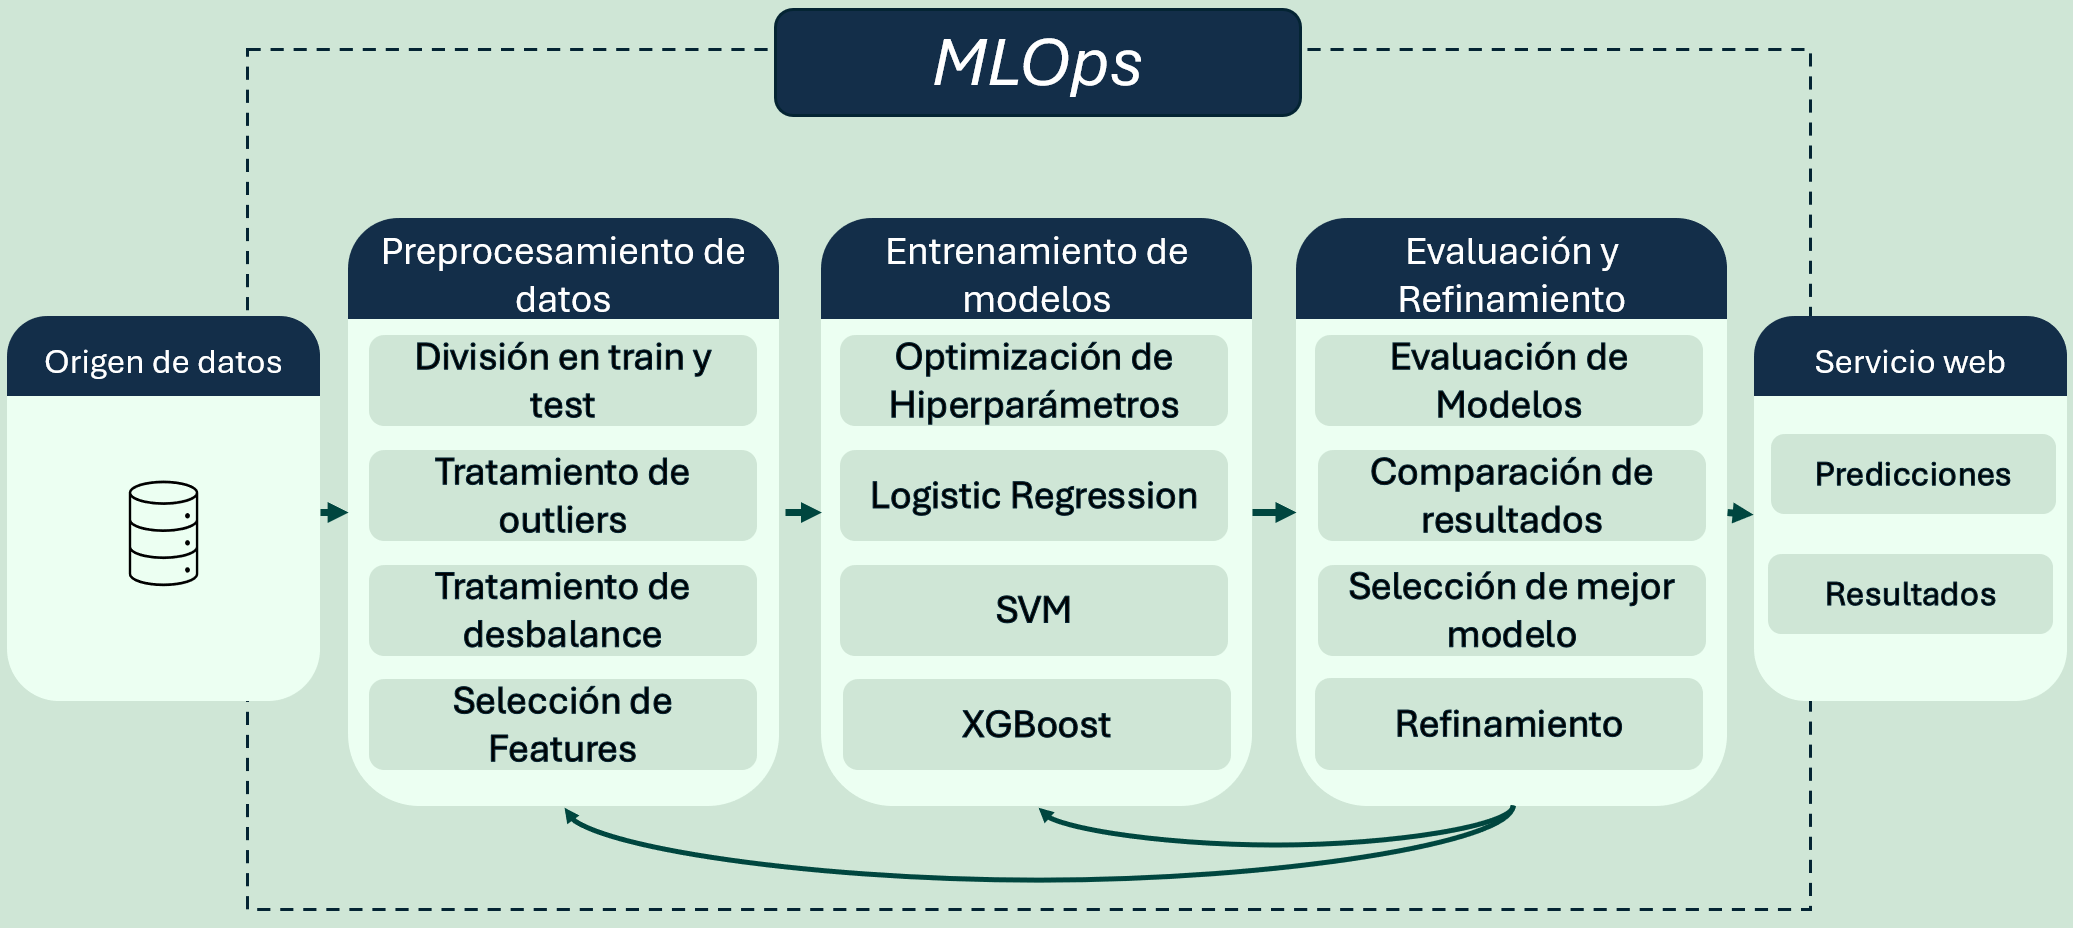
\includegraphics[width=0.9\textwidth]{./Figures/diagramaEnBloques.png}
	\caption{Flujo de trabajo utilizado.}
	\label{fig:flujo_trabajo}
\end{figure}

\subsection{Etapas del flujo de trabajo}

La primera etapa del flujo de trabajo implementado consta de la obtención del origen de datos del sistema: el dataset de \textit{Taiwanese Bankruptcy Prediction} \citep{taiwanese_bankruptcy_prediction_572}. Este es de origen público y cuenta con más de 6800 registros, que tienen información financiera de empresas del mercado de Taiwán entre 1999 y 2009.
La última etapa consiste en la publicación de un servicio web, que permitirá a los distintos usuarios realizar predicciones utilizando un modelo entrenado en este trabajo.

Entre estas dos etapas se encuentran otras que se caracterizan por ejecutarse de manera iterativa. Esto se debe a que se busca mejorar los resultados de las iteraciones anteriores, ya sea modificando algunos de sus parámetros o alterando la cantidad y/o el orden de sub-tareas dentro de cada etapa. Estas son:

\begin{itemize}
    \item Preprocesamiento de datos: en que, a grandes razgos, se mejora la calidad de dataset. Entre sus sub-tareas se encuentran la división del dataset en train y test, tratamiento de \textit{outliers}, tratamiento de desbalance y selección de \textit{features}.
    \item Entrenamiento de modelos: en que se crean, entrenan y optimizan modelos de \textit{machine learning}, utilizados para realizar predicciones de quiebra.
    \item Evaluación y refinamiento de modelos: en que se evalúan los modelos de la etapa anterior y se selecciona al mejor de ellos.
\end{itemize}

\subsection{Implementación del flujo de trabajo}

Para implementar el flujo de trabajo se optó por definir dos ambientes: un ambiente local y otro dockerizado.

El ambiente local se utiliza principalmente para experimentar distintas técnicas, herramientas e incluso sus posibles combinaciones. Por este motivo, este ambiente está constituído por \textit{notebooks} de python. Una vez determinada cuáles son las mejores técnicas y en qué orden deben ejecutarse, se procede a replicarlas en el ambiente dockerizado.

Por su parte, el ambiente dockerizado está orientado a la automatización del flujo de trabajo. De ahí a que se utilicen distintos contenedores de docker. Estos se crean para las etapas desde la descarga del dataset hasta la exposición de los modelos mediante un servicio web.

%----------------------------------------------------------------------------------------
%	SECTION 2
%----------------------------------------------------------------------------------------
\section{Arquitectura del sistema}

En la sección \ref{sec:flujo_trabajo} se describe el porqué del uso de dos ambientes al implementar el flujo de trabajo. En esta sección se describe la arquitectura de cada uno de estos ambientes. Igualmente, se remarca que en las futuras secciones y capítulos, al hablar de "sistema"\ se hará referencia al sistema desplegado mediante el ambiente dockerizado.

\subsection{Arquitectura del ambiente local}

El ambiente local se caracteriza por estar compuesto por un total de cinco directorios, cada uno dedicado a explorar distintas técnicas y/o herramientas. Cada directorio tiene una cantidad distintas de notebooks de python, que se ejecutan en el orden indicado en la figura \ref{fig:flujo_trabajo_local}. Por su parte, las notebooks generan dos datasets, uno para los datos de entrenamiento o \textit{train}, y otro para los datos de pruebas o \textit{test}. Estos datasets son a su vez utilizados como inputs por las notebooks del directorio siguiente en la secuencia de ejecución.

\begin{figure}[htbp]
	\centering
	
\includegraphics[width=0.95\textwidth]{./Figures/diagrama_componentes_local.png}
	\caption{Arquitectura del ambiente local.}
	\label{fig:flujo_trabajo_local}
\end{figure}

El primer directorio que se tiene en el ambiente local es el de análisis exploratorio. Éste, mediante la única notebook presente, se encarga de descargar el dataset original con el fin de analizarlo. En esta notebook se exploran las \textit{features} del dataset y su columna \textit{target} del dataset, haciendo foco en sus distribuciones, búsqueda de valores nulos y atípicos, como así también en la cantidad de clases presentes en la columna \textit{target}. Como esta es una notebook con fines exploratorios, el dataset de salida es el mismo que el de entrada.

El segundo directorio también consta de una sola notebook. Su objetivo es el de dividir al dataset original en un dataset de \textit{train} y otro de \textit{test}. Estos datasets nuevos constituyen la salida de este directorio, y son utilizados como entrada del siguiente.

El tercer directorio consta de dos notebooks: una para procesar datos nulos y otro para procesar \textit{outliers}. Como los datasets no tienen nulos, los datasets de salida quedan definidos por el notebook de procesamiento de \textit{outliers}.

El cuarto directorio está orientado al \textit{feature engineering}. En este se ejecutan las notebooks de escalado de datos, balanceo de datasets y selección de features de manera secuencial, generando un nuevo dataset de \textit{train} y \textit{test}.

Finalmente, en el quinto directorio se tienen tres notebooks que se ejecutan individualmente. Estas se encargan de optimizar los hiperparámetros y entrenar a los tres modelos de \textit{machine learning} utilizados en este trabajo. Finalmente, cada notebook genera un modelo distinto como salida, que se utilizan localmente para obtener métricas. A partir de estas métricas es que se decide si la ejecución total de notebooks es buena o no, y en caso de serlo, será replicada en el ambiente dockerizado.

\subsection{Arquitectura del ambiente dockerizado}

El ambiente dockerizado consta de cinco módulos principales, entre los que se encuentra el servicio web con el que los usuarios y/o interesados pueden interactuar, ya sea solicitando realizar predicciones o consultando métricas y/o gráficos. En la figura \ref{fig:flujo_trabajo_dockerizado} se puede esta arquitectura.

\begin{figure}[htbp]
	\centering
	
\includegraphics[width=0.95\textwidth]{./Figures/diagrama_componentes.png}
	\caption{Arquitectura del ambiente dockerizado.}
	\label{fig:flujo_trabajo_dockerizado}
\end{figure}

En el primer módulo se realiza la descarga del dataset, la división de \textit{train} y \textit{test}, y el preprocesamiento. Es decir, este módulo abarca las tareas realizadas en los primeros tres directorios del ambiente local.

En el segundo módulo se realiza la optimización de hiperparámetros y el entrenamiento de los modelos de \textit{machine learning}. Si bien estas dos tareas son secuenciales, las ejecuciones correspondientes a cada modelo se realizan en paralelo. Como salida se obtienen los tres modelos, que son utilizados por los módulos de \textit{tracking server} y "mejor modelo".

El módulo de "mejor modelo", como su nombre lo indica, se encarga de comparar los modelos de \textit{logistic regression}, SVM y XGBoost en función de sus métricas. A partir de esto es que se decide cuál de ellos es el mejor. Este modelo será guardado en el \textit{tracking server}, para que posteriormente puede ser utilizado por el servicio web para realizar predicciones.

El \textit{tracking server} consiste en una implementación de MLFlow. Mediante este, se tiene un servidor en donde se almacenan todas las versiones de los modelos entrenados, sus métricas, sus gráficos, como así también todas las versiones del mejor modelo. De esta manera, se puede acceder a esta información en cualquier momento.

Uno de los componentes que accede al \textit{tracking server} es el servicio web. Más precisamente, accede a la última versión del mejor modelo. También accede a las métricas y gráficos de la última versión de cada modelo entrenado. Esto le permite responder a las solicitudes de usuarios, ya sea para realizar inferencias, como también para responder consultas respecto a métricas y/o gráficas.

%----------------------------------------------------------------------------------------
%	SECTION 3
%----------------------------------------------------------------------------------------
\section{Preprocesamiento de datos}
\label{sec:preprocesamiento_de_datos}

El preprocesamiento abarca las tareas relacionadas a la división de dataset, tratamiento de nulos y de \textit{outliers}, escalado de datos, balanceo de dataset y selección de \textit{features}. A continuación se detalla en que consiste cada una de estas tareas.

\subsection{División del dataset}
\label{subsec:division_dataset}

El dataset original de \textit{Taiwanese Bankruptcy Prediction} \citep{taiwanese_bankruptcy_prediction_572} cuenta con un total de 6819 registros, entre los que hay un total de 220 casos de empresas que entran en quiebra. Si bien estos datos son suficientes para entrenar los modelos de \textit{machine learning} deseados, se presentan dos inconvenientes.

El primero es que hay un desbalance del dataset, siendo la clase objetivo mayoritaria la de empresas que no entran en quiebra. El segundo problema consiste en la necesidad de datos para evaluar qué tan bien generalizan los modelos.

Mediante la división del dataset en \textit{train} o entrenamiento y \textit{test} o evaluación se podrá resolver parte de este problema. Esto permitirá tener un set de datos reservado exclusivamente para la evaluación de modelos. Para ello, se utilizará la función \texttt{train\_test\_split} \citep{WEBSITE:train_test_split} de la biblioteca \texttt{scikit-learn} \citep{WEBSITE:scikit-learn}. Esta función además cuenta con el parámetro \texttt{stratify}, que permite dividir una clase en particular proporcionalmente entre los datasets resultantes.

Al implementar la función \texttt{train\_test\_split} se opta por generar un dataset de \textit{test} equivalente al 30\% de los datos originales, es decir, 2046 registros de un total de 6819. A su vez, mediante el parámetro \texttt{stratify}, se logra una distribución proporcional de registros de empresas en quiebra, quedando 154 para \textit{train} y 66 para \textit{test}.

\subsection{Tratamiento de nulos y outliers}

En este caso comienza buscando la presencia de datos nulos en los datasets de \textit{train} y \textit{test}. Al analizar todas las columnas de estos dataset, no se encontraron nulos, por lo que tampoco se aplican medidas de corrección.

En cuanto a los \textit{outliers} o datos atípicos, se utiliza la técnica rango intercuartil o IQR para detectarlos. Para tratarlos, se implementan las técnicas de imputación por media, imputación por mediana, imputación por moda, transformación por raíz cuadrada y transformación de Yeo-Johnson. Todas estas técnicas son explicadas en las sección \ref{subsec:tecnicas_procesamiento}.

Los cálculos del IQR y de las medidas de tendencia central (media, moda y mediana) se hicieron sobre el dataset de \textit{train}, mas no sobre el de \textit{test}. Luego, en \textit{test} se consideran \textit{outliers} a aquellos valores que no se encuentren en el IQR de \textit{text}, según cada columna, y se imputan con los valores obtenidos en \textit{train}.

Esto es para evitar que haya \textit{data leakage}, es decir, que se filtren datos o características del dataset de \textit{test} en el dataset de \textit{train}. Si esto sucediese, los modelos de \textit{machine learning} entrenados con estos dataset con datos filtrados podrían aprender indirectamente algunas de estas características, lo que evitaría que generalicen correctamente. En cuanto a la transformación por raíz cuadrada y transformación de Yeo-Johnson, estas simplemente se aplican sobre todo el rango de valores de los datasets deseados por separado.

Para definir qué técnica se aplica en cada columna, se opta por primero aplicar las cinco técnicas a cada columna. Luego, para cada técnicas, se calculan cuántos \textit{outliers} hay en la columna modificada. Finalmente, se elige a aquella técnica que haya generado la menor cantidad posible de \textit{outliers}.

Si bien este método ayuda a reducir la cantidad de datos atípicos, estos no serán siempre cero. Por ejemplo, la variable \texttt{total asset turnover} se trató con la transformación de Yeo-Johnson, que redujo los \textit{outliers} de 247 a cero, tal como se ve en la figura \ref{fig:transformacion-yeo-johnson}.

\begin{figure}[htbp]
	\centering
	
\includegraphics[width=0.95\textwidth]{./Figures/transformacion-yeo-johnson.png}
	\caption{Transformación de Yeo-Johnson sobre la columna \texttt{Total Asset Turnover}.}
	\label{fig:transformacion-yeo-johnson}
\end{figure}

Pero, para el caso de la variable \texttt{cash flow per share}, la técnica que menos \textit{outliers} genera es la de imputación por mediana, tal como se ve en la figura \ref{fig:imputacion-por-mediana}, la que reduce los \textit{outliers} de 383 a 191.

\begin{figure}[H]
	\centering
	
\includegraphics[width=0.95\textwidth]{./Figures/imputacion-por-mediana.png}
	\caption{Imputación por mediana sobre la columna \texttt{Cash Flow Per Share}.}
	\label{fig:imputacion-por-mediana}
\end{figure}

\subsection{Escalado de datos}

Las distintas columnas de los datasets presentan diferentes rangos de valores. Esto es un factor que puede perjudicar a los modelos entrenados con dichos datos, ya que pueden priorizar erróneamente una columna frente a otras solamente por esta diferencia de rangos. Por ello, es fundamental escalar los datos antes de entrenar ciertos modelos de \textit{machine learning}.

Para el escalado de datos se toma una estrategia similar a la del tratamiento de \textit{outliers}: las técnicas de escalado se ajustan en el dataset de \textit{train}, y se aplican en ambos datasets. De esta manera se evita el \textit{data leakage} en esta etapa.

En este caso solo se estudia e implementa la técnica de StandardScaler \citep{WEBSITE:standardscaler}. El beneficio se encuentra al entrenar modelos de \textit{logistic regression} y SVM, ya que permite mejorar sus reultados. Por su parte, el modelo XGBoost es más robusto a la diferencia de escalas entre columnas. Esto se puede observar en el paper de \textit{The Impact of Feature Scaling In Machine Learning: Effects on Regression and Classification Tasks} \citep{article:feature-scaling}.

El efecto se puede observar, por ejemplo, en los casos de las columnas \texttt{total expense/assets} y \texttt{retained earnings to total assets} del dataset de \textit{train}. En la figura \ref{fig:standard-scaling-01}, en el histograma de la izquierda, se observa que la primera de estas columnas tiene un rango relativamente pequeño, que va desde el cero hasta el 0,03, con media de 0,02 y desvío de 0,01.

\begin{figure}[htbp]
	\centering
	
\includegraphics[width=0.95\textwidth]{./Figures/standard-scaling-caso-01.png}
	\caption{Standard scaler aplicado a \texttt{Total expense/assets}.}
	\label{fig:standard-scaling-01}
\end{figure}

Respecto a la columna \texttt{retained earnings to total assets}, en el histograma de la izquierda de la figura \ref{fig:standard-scaling-02}, se observa que el rango original es relativamente mayor, ya que va desde el 0,91 hasta el 0,96, con media 0,94 y desvío de 0,01. Al aplicar \textit{standard scaling} a ambas columnas (por separado) se observa que los rangos ahora se encuentran entre -3 y 3 (aproximadamente) para ambos casos, teniendo ambas una media de 0 y un desvío de 1.

\begin{figure}[htbp]
	\centering
	
\includegraphics[width=0.95\textwidth]{./Figures/standard-scaling-caso-02.png}
	\caption{Standard scaler aplicado a \texttt{Retained Earnings to Total Assets}.}
	\label{fig:standard-scaling-02}
\end{figure}

\subsection{Balanceo del dataset}

Tal como se menciona en la sección \ref{subsec:division_dataset}, tanto el dataset original como los dataset resultantes al dividir en \textit{train} y \textit{test} presentan un desbalance en la columna objetivo \texttt{Bankrupt}, tal como se observa en la figura \ref{fig:descabalance-target}. Este tipo de problemas deben de resolverse antes de entrenar los modelos deseados, ya que, en caso contrario, los modelos podrían generalizar erróneamente nuevos casos.

\begin{figure}[htbp]
	\centering
	
\includegraphics[width=0.95\textwidth]{./Figures/desbalance.png}
	\caption{Desbalance de la columna Bankrupt? en el dataset de train.}
	\label{fig:descabalance-target}
\end{figure}

Para resolver el desbalance se realizan pruebas con SMOTE \citep{article:smote}, SMOTE-ENN \citep{article:smoteenn} y ADASYN \citep{article:adasyn}, técnicas que permiten generar datos sintéticos de distintas maneras, tal como se explica en la sección \ref{subsec:tecnicas_balanceo}. Como estos datos son sintéticos, las técnicas se aplican solamente en el dataset de \textit{train}, ya que aplicarlas a \textit{test} podría provocar \textit{data leakage}.

Los resultados de aplicar estas técnicas se observan en la tabla \ref{tab:resultados-balanceo}. En la misma se observa que SMOTE-ENN es la que menos registros generó, como así también la que mayor diferencia entre clases tiene (la clase positiva, o empresas que entran en quiebra, tiene 691 registros más que la otra clase). Igualmente, se opta por aplicar esta técnica en el flujo de trabajo final, ya que es la que mejor resutados arroja.

\begin{table}[H]
	\centering
	\caption[Técnicas utilizadas]{Resultados de las técnicas de balanceo de datos.}
	\begin{tabular}{c c c c c}
		\toprule
		\textbf{Técnica} 	 & \textbf{Registros nuevos} & \textbf{Clases positivas} & \textbf{Clases negativas}\\
		\midrule
        ADASYN & 9265 & 4646 & 4619 \\
        SMOTE & 9238 & 4619 & 4619  \\
        SMOTE-ENN & 8547 & 4619 & 3928 \\		
		\bottomrule
		\hline
	\end{tabular}
	\label{tab:resultados-balanceo}
\end{table}

\subsection{Selección de features}
\label{subsec:preproc_seleccion_features}

La última etapa del preprocesamiento consta de la selección de features. Mediante esta, se busca reducir la cantidad de columnas de los datasets, a modo de quedarse con aquellas que mayor información brindan sobre la columna objetivo.

Para este caso, solamente se implementa la técnica de información mutua, explicada en la sección \ref{subsec:seleccion_features}. En las primeras pruebas realizadas mediante esta técnica, se obtuvieron 66 columnas del dataset de \textit{train} que mejor explican a la variable \textit{target}. El resto de las columnas son posteriormente descartados en ambos datasets. Como el número 66 fue elegido al azar (más precisamente, se eligió al azar el 70\% de las columnas más representativas), se opta por configurar este valor representativo de la cantidad de columnas como un hiperparámetro al entrenar los distintos modelos. De esta manera, se obtiene el número que mejor resultados permita obtener en cuanto a predicciones.

Cabe aclarar que otra técnica estudiada es la de ANOVA \citep{article:anova}. Como prerequisito para aplicarla, es necesario que las distribuciones de cada columna sobre las categorías de la columna objetivo tengan distribución normal y sean homocedásticas (es decir, que tengan varianzas iguales). Como estos prerequisitos no se cumplen en el dataset de \textit{train}, se descartó el uso de la técnica de ANOVA para seleccionar features.

%----------------------------------------------------------------------------------------
%	SECTION 4
%----------------------------------------------------------------------------------------
\section{Optimización y entrenamiento de modelos}
\label{sec:optimizacion_y_training}

Una vez preprocesado el dataset original y generados los datasets de \textit{train} y \textit{test}, se comienza con el entrenamiento de modelos. A fin de generar los mejores modelos, se procede a optimizar sus hiperparámetros, como así también se realizan pruebas utilizando \textit{pipelines}.

\subsection{Pipelines y modelos}
\label{sec:pipelines_y_modelos}

En este trabajo se realizaron distintas pruebas con modelos de \textit{machine learning}. En todas estas, el preprocesamiento aplicado era el descrito en la sección \ref{sec:preprocesamiento_de_datos}, es decir, una serie de técnicas que, aplicadas sobre el dataset original, generaban un dataset final de \textit{train} y otro de \textit{test}. Luego, estos dataset se utilizan como \textit{input} de los modelos, tanto para entrenarlos como para evaluarlos. Pero ciertos modelos no presentaban buenos resultados. Un ejemplo es XGBoost, que en ciertas pruebas arroja un \textit{recall} de 0,42, un valor muy bajo.

Para mejorar esto, se utiliza la clase \texttt{Pipeline} \citep{WEBSITE:imblearn-pipeline} de \texttt{Imblearn} \citep{WEBSITE:imblearn}. Tal como su nombre lo indica, permite generar un \textit{pipeline} o secuencia de pasos sobre un dataset a fin de ajustarlo, y posteriormente transformar o aplicar los pasos tanto en este como en otros datasets. Las ventajas que poseen estos \textit{pipelines} es que procesan mejor los datos de datasets desbalanceados, manejan mejor el \textit{cross-validation} con \textit{resampling} (técnica que se explica posteriormente) y está específicamente diseñado para usarse al optimizar hiperparámetros.

A nivel implementación, el \textit{pipeline} utilizado consta de los mismos pasos definidos en el preprocesamiento: correción de datos atípicos, escalado, balanceo de datos y selección de features. Se agrega también un paso final correspondiente al entrenamiento del modelo, ya que mejoran los resultados tanto al entrenar como al optimizar hiperparámetros. Luego, mediante el método \texttt{fit} junto al dataset de \textit{train}, aplica las transformaciones a los datos y entrena al modelo, mientras que con el método \texttt{predict} junto al dataset de \textit{test} evalúa al modelo final.

En cuanto a resultados, la misma secuencia de transformaciones que se utilizaron para el modelo XGBoost y dieron un resultado para \textit{recall} de 0,42, con la implementación de la clase \texttt{Pipeline} dieron un \textit{recall} de 0,8. Por este motivo, se opta por utilizar \textit{pipelines} para entrenar y optimizar modelos.

\subsection{Cross validation e implementación durante optimización}

Con el fin de optimizar hiperparámetros se utiliza el \textit{framework} \texttt{optuna} \citep{article:optuna}. Este se caracteriza por utilizar optimización bayesiana \citep{artice:bayesion-optimization}, que permite determinar qué combinaciones de parámetros funcionarán mejor basándose en resultados anteriores, lo que permite ahorrar tiempo de cómputo.

Esta herramienta fue combinada con la técnica de \textit{cross validation}, que permite dividir el dataset en k subconjuntos o \textit{folds} iguales, con el fin de realizar k entrenamientos. Más precisamente, se utiliza un fold distinto para validar y el resto para entrenar. En particular, se utiliza la función \texttt{cross\_validate} \citep{WEBSITE:crossvalidate} de \texttt{scikit-learn} \citep{WEBSITE:scikit-learn}.

Este enfoque asegura que cada configuración de hiperparámetros sea evaluada de manera exhaustiva en diferentes subconjuntos de datos, lo que a su vez permite prevenir el \textit{overfitting} y mitigar el \textit{data leakage}. También permite obtener una estimación robusta del entrenamiento, ya que se promedian los resultados de los k experimentos.

En este trabajo se opta por utilizar 5 folds, entrenados durante 100 iteraciones de \texttt{optuna}. Esto se implementa mediante la clase \texttt{StratifiedKFold} \citep{WEBSITE:stratifiedkfold}, que mediante el parámetro \texttt{shuffle} permite mezclar los datos para evitar sesgos.

Otra herramienta utilizada es \texttt{MedianPruner} \citep{WEBSITE:MedianPruner}, que permite realizar una exploración más profunda del espacio de búsqueda en menor tiempo. Esto lo logra al detener automáticamente los ensayos cuyos resultados preliminares, es decir, durante los primeros folds de la validación cruzada, no superan la mediana de rendimiento de intentos anteriores.

Finalmente, a la hora de optimizar mediante \texttt{optuna}, se busca maximizar la métrica de AUPRC. Esta métrica es ideal ya que, tal como se menciona en el paper \textit{A closer look at AUROC and AUPRC under class imbalance} \citep{article:closer_look_auprc}, es ideal para utilizar en casos en que existe desbalanceo de clases. En particular, esta métrica se obtiene al configurar el parámetro \texttt{scoring} de \texttt{cross\_validate} con el valor \texttt{average\_precision} \citep{WEBSITE:scikit_learn_scoring_names} (internamente utiliza \texttt{average\_precision\_score} \citep{WEBSITE:average_precision_score}).

\subsection{Modelo Logistic Regression}
\label{subsec:cap3_models_lr}

El primer modelo que se utiliza en este trabajo es la regresión logística o \textit{Logistic Regression} \citep{model:lr}. Se lo elige principalmente para utilizarlo como modelo \textit{baseline}, es decir, para definir una base de rendimiento antes de utilizar otros modelos más complejos. Igualmente, este modelo presenta ciertos beneficios, como ser computacionalmente económico y rápido para entrenar, o estar diseñado para devolver probabilidades bien calibradas.

Se implementa con la clase \texttt{LogisticRegression} \citep{WEBSITE:sklearn_LogisticRegression} de \texttt{scikit-learn}. En particular, se optimizan los siguientes hiperparámetros:

\begin{itemize}
    \item \texttt{C} o fuerza de regularización: controla el equilibrio entre ajustar bien los datos y evitar el sobreajuste. Mediante \texttt{optuna} se explora el rango entre $1e^{-5}$ y $1e^2$.
    \item \texttt{Penalty} o penalización: determina qué tipo de regularización utilizar. \texttt{L1} (Lasso) es excelente para selección de variables, mientras que \texttt{L2} (Ridge) es el estándar para estabilidad. Se exploran ambos valores posibles.
    \item \texttt{solver} o algoritmo de optimización: determina el algoritmo a utilizar. Se utiliza \texttt{liblinear}.
    \item \texttt{max\_iter} o máximo de iteraciones: es el número de pasos que da el algoritmo para converger. Se utiliza el valor $1000$.
    \item \texttt{tol} o tolerancia: define el criterio de parada. Si la mejora entre iteraciones es menor a este valor, el modelo deja de entrenar. Ayuda a evitar cómputo innecesario cuando el modelo ya es estable. Se explora el rango entre los valores $1e^{-6}$ y $1e^{-3}$.
\end{itemize}

Durante la optimización también se busca determinar la cantidad de \textit{features} a elegir para la técnica de información mutua, tal como se expresa en \ref{subsec:preproc_seleccion_features}. No solamente se busca cuál es el mejor valor, sino cuál es la mejor manera. Entre estas, se estudian:

\begin{itemize}
    \item Elección de un porcentaje de \textit{features}: utiliza la clase \texttt{SelectPercentile} \citep{WEBSITE:sklearn_SelectPercentile}. Para ello se define el parámetro \texttt{percentile}, y se explora en el rango $50$ y $80$, es decir, entre el 50\% y 80\%.
    \item Elección de una cantidad fija: se logra mediante la clase \texttt{SelectKBest} \citep{WEBSITE:sklearn_SelectKBest}. Se define el parámetro \texttt{k\_features}, que se explora en el rango $15$ y $80$.
\end{itemize}

Los valores encontrados en el proceso de optimización se listan en la tabla \ref{tab:log-reg-hip}.

\begin{table}[h]
	\centering
	\caption[Hiperparámetros - LR]{Hiperparámetros optimizados para Logistic Regression.}
	\begin{tabular}{c c}
		\toprule
		\textbf{Hiperparámetro} 	 & \textbf{Mejor valor encontrado} \\
		\midrule
        \texttt{C} & $0,0213370341121205$\\
        \texttt{penalty} & \texttt{L1} (Lasso) \\
        \texttt{solver} & \texttt{liblinear} \\
        \texttt{max\_iter} & $1000$ \\
        \texttt{tol} & $0,00013579751380015856$ \\
        Selección de features & \texttt{SelectPercentile} \\
        \texttt{percentile} &  $79$ \\
		\bottomrule
		\hline
	\end{tabular}
	\label{tab:log-reg-hip}
\end{table}

\subsection{Modelo SVM}

El siguiente modelo utilizado es el \textit{Support Vector Machine} o SVM \citep{model:svm}. Este modelo es eficiente en espacios de alta dimensionalidad como el del dataset de estudio, que cuenta con un total de $95$ \textit{features}, ya que busca el hiperplano óptimo basándose solo en los puntos más críticos. También se caracteriza por el manejo de relaciones no lineales, lo que es ideal para este trabajo, ya que la relación entre los ratios financieros y la quiebra no siempre es lineal. Otra ventaja es que es un modelo robusto frente al \textit{overfitting}, ya que maximiza la distancia entre las clases, lo que tiende a generalizar mejor en datos no vistos. Por último, estudios como \textit{Financial Distress Prediction Using Support Vector Machines and Logistic Regression} \citep{article:financial_distress_svm} remarcan que estos modelos presentan buenos resultados en problemas de predicción/clasifiación de quiebra y/o problemas financieros.

Respecto a su implementación, se utiliza la clase \texttt{SVC} \citep{WEBSITE:sklearn_SVC} de \texttt{scikit-learn}, que consiste en una implementación de SVM para problemas de clasificación. Esto nos permite explorar los siguientes hiperparámetros:

\begin{itemize}
    \item \texttt{C} o parámetro de regularización: controla el equilibrio entre maximizar el margen del hiperplano y minimizar el error de clasificación en el entrenamiento. Se exploran los valores dentro del rango $1e^{-5}$ y $1e^{2}$.
    \item \texttt{kernel} o función de núcleo: define el tipo de frontera de decisión para transformar los datos. Se exploran los valores \texttt{linear}, \texttt{poly}, \texttt{rbf} y \texttt{sigmoid}.
    \item \texttt{gamma} o coeficiente del kernel: define cuánto alcance tiene la influencia de un solo ejemplo de entrenamiento. Solo aplica para kernels \texttt{poly}, \texttt{rbf} y \texttt{sigmoid}. Se estudian los valores dentro del rango  $1e^{-4}$ y $1$.
\end{itemize}

De la misma manera que en la sección \ref{subsec:cap3_models_lr}, se exploran los hiperparámetros para determinar la cantidad óptima de \textit{features} para la selección mediante \textit{mutual information}.

Los mejores hiperparémtros encontrados para SVC se listan en la tabla \ref{tab:svm-hip}.

\begin{table}[h]
	\centering
	\caption[Hiperparámetros - SVM]{Hiperparámetros optimizados para SVM.}
	\begin{tabular}{c c}
		\toprule
		\textbf{Hiperparámetro} 	 & \textbf{Mejor valor encontrado} \\
		\midrule
        \texttt{C} & $0,009090342537573116$ \\
        \texttt{kernel} & \texttt{linear} \\
        \texttt{gamma} & $0,0001223840354008705$ \\
        Selección de features & \texttt{SelectPercentile} \\
        \texttt{percentile} &  $68$ \\
		\bottomrule
		\hline
	\end{tabular}
	\label{tab:svm-hip}
\end{table}

\subsection{Modelo XGBoost}

El último modelo estudiado es XGBoost \citep{model:xgboost}. Este es un algoritmo de \textit{ensemble learning} basado en árboles de decisión que construye modelos de forma secuencial para corregir los errores de los anteriores. Esto hace que, en problemas con datos estructurados (como los de este trabajo), supere consistentemente a otros algoritmos. Otro de los motivos de su elección es que ayuda a prevenir el \textit{overfitting}, ya que incluye penalizaciones L1 (Lasso) y L2 (Ridge) en su función objetivo. Finalmente, este algoritmo presenta el parámetro \texttt{scale\_pos\_weight}, que permite tratar el desbalance al dar más peso a una clase minoritaria, lo que resulta ideal para el dataset utilizado.

Desde el punto de vista técnico, se utiliza la clase \texttt{XGBClassifier} \citep{WEBSITE:xgboost_classifier} del package \texttt{xgboost} \citep{WEBSITE:package_xgboost}. Esta permite utilizar los siguientes hiperparámetros:

\begin{itemize}
    \item \texttt{max\_depth} o profundidad máxima: determina qué tan complejo y profundo puede ser cada árbol. Valores altos capturan relaciones más complejas pero aumentan el riesgo de \textit{overfitting}. Se estudia el rango entre $2$ y $10$.
    \item \texttt{min\_child\_weight}: define la suma mínima de pesos necesaria en un nodo para crear una nueva partición. Es una de las herramientas más potentes para controlar el sobreajuste: valores altos hacen que el modelo sea más conservador. Se estudian los valores entre $1$ y $10$.
    \item \texttt{subsample} o submuestreo de filas: fracción de datos de entrenamiento que se muestrea aleatoriamente para construir cada árbol. Ayuda a prevenir el sobreajuste al introducir aleatoriedad. Se estudian los valores entre $0,6$ y $1$.
    \item \texttt{colsample\_bytree} o submuestreo de columnas: fracción de las 95 variables financieras que se seleccionan para cada árbol. Se estudia el rango entre $0,2$ y $1$.
    \item \texttt{learning\_rate} o tasa de aprendizaje: controla qué tan rápido aprende el modelo. El rango estudiado es $0,001$ y $0,1$.
    \item \texttt{reg\_alpha} o penalización L1: permite regularizar los pesos de las hojas. Se estudia el rango entre $0$ y $10$.
    \item \texttt{reg\_lambda} o penalización L2: permite regularizar los pesos de las hojas. Se estudia el rango entre $0$ y $10$.
    \item \texttt{n\_estimators} o cantidad de estimadores: representa el número total de árboles de decisión que se construirán secuencialmente. El espacio de búsqueda se define entre $100$ y $1000$.
    \item \texttt{gamma}: especifica la pérdida mínima requerida para realizar una partición adicional en un nodo del árbol. A mayor gamma, más conservador es el algoritmo. Se estudian los valores entre $0$ y $5$.
\end{itemize}

De la misma manera que en la sección \ref{subsec:cap3_models_lr}, se exploran los hiperparámetros para determinar la cantidad óptima de \textit{features} para la selección mediante \textit{mutual information}.

Los mejores hiperparamétros encontrados para XGBoost se listan en la tabla \ref{tab:xgboost-hip}.

\begin{table}[ht]
	\centering
	\caption[Hiperparámetros - XGBoost]{Hiperparámetros optimizados para XGBoost.}
	\begin{tabular}{c c}
		\toprule
		\textbf{Hiperparámetro} 	 & \textbf{Mejor valor encontrado} \\
		\midrule
        \texttt{max\_depth} & $10$ \\
        \texttt{min\_child\_weight} & $3$ \\
        \texttt{subsample} & $0,6$ \\
        \texttt{colsample\_bytree} & $0,5$ \\
        \texttt{learning\_rate} & $0,1$ \\
        \texttt{reg\_alpha} & $0,1$ \\
        \texttt{reg\_lambda} & $5$ \\
        \texttt{n\_estimators} & $700$ \\
        \texttt{gamma} & $3,9311947393215356$ \\
        Selección de features & \texttt{SelectPercentile} \\
        \texttt{percentile} &  $75$ \\
		\bottomrule
		\hline
	\end{tabular}
	\label{tab:xgboost-hip}
\end{table}

\subsection{Selección del mejor modelo}

Luego de optimizar los hiperparámetros y entrenar a cada modelo, se obtienen métricas de \textit{recall}, \textit{precision}, \textit{f1-score}, \textit{f2-score}, AUC-ROC y \textit{average precision}. Estas se registran en el \textit{tracking server} para poder ser utilizadas en pasos posteriores.

Uno de estos pasos es el de la selección del mejor modelo. El proceso es simple: se ordenan los modelos en función de una métrica configurada, y se selecciona al que presenta mejor valor.

En la configuración actual del trabajo se utiliza la métrica de \textit{average precision}, misma métrica que se usa para optimizar hiperparámetros. Esta define como mejor modelo a XGBoost.

%----------------------------------------------------------------------------------------
%	SECTION 5
%----------------------------------------------------------------------------------------
\section{Tracking server}

En este trabajo se realizaron varias iteraciones sobre sus distintas etapas, principalmente en la de optimización y entrenamiento de modelos (sección \ref{sec:optimizacion_y_training}). Como resultado de cada iteración se obtienen: tres modelos nuevos (\textit{Logistic Regression}, SVM y XGBoost), un conjunto de hiperparámetros óptimos para cada modelo, un conjunto de métricas de para cada uno de ellos y, finalmente, un mejor modelo, o modelo ganador/\textit{champion}.

Estos objetos generados son utilizados en etapas posteriores. Por ejemplo, el servicio web utiliza el modelo ganador para realizar predicciones, como así también accede a las métricas de los modelos ante distintas consultas de los usuarios. Por este motivo, resulta fundamental tener un registro de todos los resultados obtenidos.

A partir de esto surge la necesidad de utilizar un \textit{tracking server} que permita almacenar estos recursos, hacer seguimiento de los cambios y comparar los resultados obtenidos.

Por estos motivos se utiliza \texttt{MLFlow} \citep{WEBSITE:mlflow}, una plataforma de código abierto que permite gestionar el ciclo de vida de los modelos entrenados. Esta herramienta cuenta tanto con un \textit{tracking server} \citep{WEBSITE:mlflow_tracking_server} como con un \textit{model registry} \citep{WEBSITE:mlflow_model_registry}, los que pueden ser utilizados mediante un paquete de Python. La diferencia entre el \textit{model registry} y el \textit{tracking server} es que este último se enfoca más en la experimentación, mientras que el primero se enfoca más en la gobernanza y producción.

El \textit{tracking server} permite guardar los resultados de cada experimento. Cada experimento se administra con una \textit{run} o ejecución, en donde se guardan los modelos en sí, sus parámetros, sus métricas y algunos gráficos. Esto se logra mediante la clase \texttt{mlflow} \citep{WEBSITE:mlflow_api} del paquete python, la que tiene los siguientes métodos:

\begin{itemize}
    \item \texttt{start\_run}: permite comenzar una \textit{run}, como así también grabar cierta información de la misma.
    \item \texttt{log\_model}: permite guardar el modelo obtenido en un experimento.
    \item \texttt{log\_params}: graba los parámetros utilizados por el modelo en una \textit{run} determinada.
    \item \texttt{log\_metrics}: graba las métricas obtenidas por un modelo en una \textit{run} determinada.
    \item \texttt{log\_figure}: graba gráficos asociados a un modelo, en una \textit{run} determinada.
\end{itemize}

Respecto al \textit{model registry}, este permite registrar aquellos modelos que se utilizan en la versión productiva del trabajo, es decir, los mejores modelos o \textit{champions}. Técnicamente, se logra mediante la clase \texttt{mlflow.client} \citep{WEBSITE:mlflow_client_api}, con los siguientes métodos:
\begin{itemize}
    \item \texttt{create\_registered\_model}: crea el registro del modelo.
    \item \texttt{set\_registered\_model\_alias}: permite poner un alias al modelo. En este trabajo el alias para todos los modelos registrados es \textit{champion}.
    \item \texttt{get\_registered\_model}: permite leer el modelo. Esto resulta ideal para realizar predicciones con el mismo.
\end{itemize}

%----------------------------------------------------------------------------------------
%	SECTION 6
%----------------------------------------------------------------------------------------
\section{Automatización mediante Airflow}
\label{sec:automatizacion_airflow}

Una vez definidos el preprocesamiento de datos, los modelos a utilizar, sus hiperparámetros y el \textit{tracking server}, se procede a automatizar la interacción entre estos.

Para esto se utiliza \texttt{airflow} \citep{WEBSITE:airflow}, un paquete de python que actúa como orquestador del flujo de trabajo. Este permite definir DAGs o \textit{directed acyclic graph} \citep{WEBSITE:airflow_dags}, un grafo acíclico dirigido donde cada nodo representa las tareas de un determinado flujo, mientras que las aristas marcan el orden de ejecución. En particular, se definieron dos DAGs.

\subsection{DAG - download and split dataset}

El primer DAG definido es \texttt{download\_and\_split\_dataset}, el que se observa en la figura \ref{fig:dag01}. Su propósito es el de descargar el dataset \textit{Taiwanese Bankruptcy Prediction} y hacer su división en \textit{train} y \textit{test}.

\begin{figure}[htbp]
	\centering
	
\includegraphics[width=0.95\textwidth]{./Figures/dag_download_and_split_dataset.png}
	\caption{DAG - download and split dataset}
	\label{fig:dag01}
\end{figure}

Para esto, se divide el DAG en dos tareas, las que se ejecutan secuencialmente:

\begin{itemize}
    \item \texttt{download\_and\_load\_dataset}: descarga el dataset original y lo guarda en una base de datos S3 (que se encuentra dockerizado).
    \item \texttt{split\_raw\_dataset}: toma el dataset original de S3 y lo divide en \textit{train} y \textit{test}. Finalmente, guarda estos dos datasets nuevos para ser utilizados en otros DAGs.
\end{itemize}

\subsection{DAG - model training}
\label{sec:model_training}
El segundo DAG es \texttt{model\_training}, el que se observa en la figura \ref{fig:dag02}. Su propósito es optimizar los hiperparámetros de los modelos, entrenar los modelos y finalmente elegir al mejor de ellos.

\begin{figure}[htbp]
	\centering
	
\includegraphics[width=0.95\textwidth]{./Figures/dag_model_training.png}
	\caption{DAG - model training.}
	\label{fig:dag02}
\end{figure}

Este DAG se caracteriza por ejecutar tres tareas en paralelo, que convergen en una tarea final. Cada una de estas leen los dataset de \textit{train} y \textit{test} originados en el DAG anterior.

Las tareas que se ejecutan en paralelo, que a su vez ejecutan internamente dos tareas secuenciales, son los siguientes:

\begin{itemize}
    \item \texttt{logistic\_regression\_training}: se encarga de optimizar los hiperparámetros de \textit{Logistic Regression} (mediante la subtarea \texttt{optimizar\_lr}) y posteriormente de entrenar dicho modelo (subtarea \texttt{entrenar\_lr}). Los resultados de cada subtarea se guardan tanto en S3 como en el \textit{tracking server} de \texttt{MLFlow}.
    \item \texttt{svm\_training}: mediante \texttt{optimizar\_svm} y \texttt{entrenar\_svm}, optimiza y entrena un modelo SVM. Sus resultados se guardan tanto en S3 como en el \textit{tracking server} de \texttt{MLFlow}.
    \item \texttt{xgboost\_training}: de manera similar a las otras tareas de este DAG, tiene una subtarea que optimiza los hiperparámetros (\texttt{optimizar\_xgboost}) y otra que entrena (\texttt{entrenar\_xgboost\_classifier}) un modelo XGBoost. Los resultados se guardan tanto en S3 como en el \textit{tracking server} de \texttt{MLFlow}.
\end{itemize}

Una vez terminadas, se ejecuta la tarea final \texttt{seleccionar\_champion}. Esta lee los modelos desde el \textit{tracking server} de \texttt{MLFlow}, los compara mediante la métrica de \texttt{average\_precision} y al mejor de estos lo guarda en el \textit{model registry} de \texttt{MLFlow} como modelo \textit{champion}.

\subsection{Configuración mediante YAML}

Para poder configurar el comportamiento de estos DAGs de \texttt{airflow}, se decide utilizar archivos \texttt{yaml} \citep{WEBSITE:yaml}. Estos se leen al comienzo de cada tarea del DAG y permiten definir, por ejemplo, qué métrica se utiliza para optimizar hiperparámetros, qué metrica se utiliza para comparar modelos, con qué nombres se guardan los modelos en \texttt{mlflow}, entre varios otros detalles.

Uno de las más importantes es la configuración de hiperparámetros de cada modelo. El archivo \texttt{yaml} permite pasar valores de pruebas realizadas en otros contextos, por ejemplo, mediante \textit{notebooks} de Python. De esta manera, en las subtareas de optimización, se evita ejecutar la optimización en sí y directamente se cargan estos datos. El motivo principal se debe a que, al utilizar \texttt{airflow} mediante \texttt{docker}, la ejecución de cada DAG demora mucho tiempo. Esto puede deberse a las especificaciones de la máquina con la que se desarrolla este trabajo (Windows 10, 12 GB de RAM), como así también a cómo \texttt{airflow} maneja internamente sus subprocesos.

%----------------------------------------------------------------------------------------
%	SECTION 7
%----------------------------------------------------------------------------------------
\section{Servicio web}

El servicio web se implementa mediante el framework FastAPI \citep{WEBSITE:fastapi}. Este consta de los siguientes endpoints:

\begin{itemize}
    \item \texttt{get\_champion\_image}: método \texttt{get} que permite obtener una imagen asociada al modelo \textit{champion} actual. Las imágenes disponibles corresponden a la matriz de confusión, matriz de confusión normalizada por fila, curva ROC y curva \textit{precision-recall}. Solamente se devuelve de a una imagen por petición.
    \item \texttt{get\_champion\_metrics}: método \texttt{get} que permite obtener las métricas del modelo \textit{champion} actual. Estas métricas incluyen \textit{precision}, \textit{recall}, \textit{f1-score}, \textit{f2-score}, AUC-ROC y \textit{average precision}.
    \item \texttt{get\_experiment\_image}: método \texttt{get} que permite obtener una imagen asociada a cualquiera de las últimas versiones de los modelos entrenados, siendo estos \textit{logistic regression}, SVM y XGBoost. Devuelve el mismo tipo de imágenes que el método \texttt{get\_champion\_image}.
    \item \texttt{get\_experiment\_metrics}: método \texttt{get} que permite obtener las métricas de las últimas versiones entrenadas de \textit{logistic regression}, SVM y XGBoost. Son las mismas métricas que devuelve \texttt{get\_champion\_metrics}.
    \item \texttt{predict}: método \texttt{post} que permite realizar predicciones a partir de los datos enviados por un usuario.
\end{itemize}

Internamente, este servicio web accede al \textit{tracking server} y al \textit{model registry} de \texttt{mlflow}. De esta manera, puede utilizar el modelo \textit{champion} para realizar predicciones e incluso para obtener métricas y gráficos. También accede a la última versión entrenada de cada modelo, con el fin de obtener métricas y gráficos. No realiza predicciones con estos.

Respecto al método \texttt{predict}, este recibe una petición del usuario con un total de 95 parámetros, correspondientes a cada \textit{feature} del dataset estudiado. Para facilitar la validación de cada una de estas, se utiliza la biblioteca de \texttt{pydantic} \citep{WEBSITE:pydantic}. Especificamente, se utilizan las clases \texttt{BaseModel} \citep{WEBSITE:pydantic_base_model}, que facilita la conversión de una petición de un usuario a una clase propia, y la clase \texttt{Field} \citep{WEBSITE:pydantic_field}, que permite definir atributos a cada uno de los campos de una clase. Luego, se define una clase propia \texttt{CompanyRequest},que contiene 95 campos que representan las \textit{features} del dataset. Esta clase implementa \texttt{BaseModel} para leer fácilmente las peticiones del usuario al método \texttt{predict}. Además, mediante \texttt{Field}, define los rangos numéricos de cada campo, lo que facilita sus validaciones.
\chapter{Ensayos y resultados} % Main chapter title

\label{Chapter4}

En este capítulo se detalla, en primer lugar, cómo se evalúan los modelos estudiados en este trabajo. Luego, se explica cómo se evalúa el entorno de Airflow, con énfasis en los dos DAGs implementados. Posteriormente, se describen las pruebas realizadas en el servicio web y se presentan cada uno de sus \textit{endpoints}. Finalmente, se detalla una prueba realizada con otro dataset.

\definecolor{mygreen}{rgb}{0,0.6,0}
\definecolor{mygray}{rgb}{0.5,0.5,0.5}
\definecolor{mymauve}{rgb}{0.58,0,0.82}

%----------------------------------------------------------------------------------------
%	SECTION 1
%----------------------------------------------------------------------------------------
\section{Evaluación de modelos}
\label{sec:pruebas_indiv_modelos}

Una vez entrenados, se evalúan los modelos y sus versiones con el fin de encontrar al mejor de todos ellos. A continuación se detallan las métricas utilizadas como así también el proceso de comparación entre modelos.

\subsection{Métricas de modelos}
En este trabajo se estudian los modelos de Logistic Regression, SVM y XGBoost. Tal como se explica en la sección \ref{sec:flujo_trabajo}, en cada una de las iteraciones de estudio se genera una nueva versión de estos modelos. Esto aplica tanto a los modelos individuales como en los basados en \textit{pipelines}, tal como se describe en la sección \ref{sec:pipelines_y_modelos}.

Debido a la gran cantidad de versiones de modelos creados, surge la necesidad de definir métricas que permitan determinar cuál de estos es el que mejor permite predecir si una empresa entra en quiebra. En la tabla \ref{tab:metricas-de-modelos} se detallan las métricas utilizadas en este trabajo.

\begin{table}[H]
    \centering
    \caption{Métricas de modelos.}
    \begin{tabularx}{\textwidth}{l X X}
        \toprule
        \textbf{Métrica} & \textbf{¿Qué mide?} & \textbf{¿Por qué se eligió?} \\
        \midrule
        Recall & Capacidad para identificar todos los casos de quiebra reales. & Minimiza los falsos negativos en riesgos financieros. \\
        Precision & Exactitud de predecir quiebra. & Evita dar falsas alarmas. \\
        F1-Score & Balance entre Precision y Recall. & Evaluación general en una sola métrica. \\
        F2-Score & Balance que prioriza el Recall. & Prioriza detección de quiebras. \\
        AUPRC & Área bajo la curva de Precision y Recall. & Métrica robusta para datasets con clases minoritarias. \\
        ROC-AUC & Capacidad de discriminar entre clases. & Evalúa el modelo globalmente. \\
        \bottomrule
		\hline
    \end{tabularx}
    \label{tab:metricas-de-modelos}
\end{table}

En la tabla \ref{tab:resultados-metricas} se muestran las métricas obtenidas para los modelos Logistic Regression, SVM y XGBoost, tanto de sus versiones individuales como aquellas basadas en \textit{pipelines}. En esta se observa que los resultados obtenidos en las versiones correspondientes a \textit{pipelines} son, en general, superiores a las versiones individuales. En función de los valores obtenidos de ROC-AUC, f2-Score y \textit{recall} se seleccionan a las versiones basadas en \textit{pipelines} para cada uno de los modelos.

\begin{table}[H]
    \centering
    \caption{Resultados de métricas de modelos.}
    \begin{tabularx}{\textwidth}{c X c X X c X}
		\toprule
		\textbf{Modelo} & \textbf{Recall} & \textbf{Precision} & \textbf{F1-Score} & \textbf{F2-Score} & \textbf{AUPRC} & \textbf{ROC-AUC}\\
		\midrule
        Logistic Regression & 0,6818 & 0,1480 & 0,2432 & 0,3961 & 0,2321 & 0,9009 \\
        LR - Pipeline & 0,8636 & 0,1347 & 0,2331 & 0,4148 & 0,2615 & 0,9181 \\
        SVM & 0,0303 & 0,1428 & 0,05 & 0,0359 & 0,2158 & 0,8854 \\
        SVM - Pipeline & 0,8181 & 0,1436 & 0,2443 & 0,4218 & 0,2405 & 0,9101 \\
        XGBoost & 0,4242 & 0,3544 & 0,3862 & 0,4081 & 0,3327 & 0,9047 \\
        XGBoost - Pipeline & 0,7727 & 0,2170 & 0,3388 & 0,5110 & 0,3388 & 0,9236 \\
        \bottomrule
		\hline
    \end{tabularx}
    \label{tab:resultados-metricas}
\end{table}

\subsection{Comparación entre modelos}

Una vez obtenidas las métricas de los modelos, se procede a compararlos entre sí. Para ello, se hace uso de la métrica AUPRC o \textit{average precision}. Por este motivo, si se observa la tabla \ref{tab:resultados-metricas}, el mejor modelo es XGBoost - pipeline.

El \textit{model registry} de MLFlow se utiliza para seleccionar el modelo correcto. En este, se registran las distintas versiones del modelo final del trabajo, cuyo nombre es \texttt{bankruptcy\_prediction}. En sus metadatos se indica qué \textit{run} o ejecución lo generó. Tal como se observa en la figura \ref{fig:best-model}, en la versión número 4 del modelo final se detalla que se genera a partir de XGBoost, lo que indica que la comparación entre modelos funciona correctamente.

\begin{figure}[H]
	\centering
	
\includegraphics[width=0.88\textwidth]{./Figures/best_model.png}
	\caption{Mejor modelo - \textit{Model registry} de MLFLow.}
	\label{fig:best-model}
\end{figure}

\subsection{Matriz de confusión normalizada del mejor modelo}

La figura \ref{fig:matriz-confusion-mejor-modelo} corresponde a la matriz de confusión normalizada por fila del mejor modelo (XGBoost - pipeline). Esta permite conocer qué tan bien clasifica el modelo a los casos de quiebra como así también a los casos de empresas sanas.

La matriz indica que el modelo obtiene un \textit{recall} o \textit{true positive rate} de $0,79$, es decir, que el modelo detecta de manera satisfactoria al $79\%$ de las empresas que entran en quiebra. El $13\%$ que resta se clasifica de manera errónea, es decir, el modelo indica que no entra en quiebra. Esto se ve en el valor de \textit{false negative rate}, que es de $0,21$.

En lo que respecta a las empresas sanas, el modelo detecta con éxito al $91\%$, tal como lo indica el \textit{true negative rate} o \textit{specifity} de $0,91$. El $9,4\%$ de casos que restan se clasifican de manera equivocada como quiebras, lo que se refleja en el \textit{false positive rate} de $0,094$.

En resumen, esta matriz describe de manera simple qué tan bien identifica el modelo a cada clase. Para el caso particular del dataset de Taiwán, la matriz indica que el modelo detecta el $79\%$ los casos de quiebra. Esta es una buena métrica, ya que el objetivo de este modelo es minimizar las quiebras no detectadas ($21\%$), debido al elevado riesgo financiero que supone un impago. Como contraparte, el modelo tiene una tasa de falsos positivos de $9,4\%$, que representan a empresas sanas marcadas como quiebra.

\begin{figure}[H]
	\centering
	
\includegraphics[width=0.95\textwidth]{./Figures/fig_matriz_confusion.png}
	\caption{Matriz de confusión del mejor modelo.}
	\label{fig:matriz-confusion-mejor-modelo}
\end{figure}

En lo que respecta al valor de falsos negativos ($21\%$), el modelo podría clasificarlos de manera errónea por razones ajenas a las variables financieras, por ejemplo, cambio en regulaciones financieras del mercado de Taiwán, crisis inesperadas, entre otras.

\subsection{Curva ROC del mejor modelo}

La figura \ref{fig:fig_roc_curve} muestra la curva ROC del mejor modelo. Esta grafica el \textit{recall} o \textit{true positive rate} del modelo contra el \textit{false positive rate} en distintos umbrales o \textit{thresholds}, que muestran la disyuntiva de identificar de manera correcta un caso positivo y marcar de manera errónea los negativos. El área bajo esta curva (AUC-ROC) permite determinar qué tan bien el modelo separa las clases. Un valor cercano a $1$ indica que se tiene un buen modelo, mientras que un valor cercano a $0,5$ muestra que el modelo tiene un comportamiento azaroso.

\begin{figure}[H]
	\centering
	
\includegraphics[width=0.92\textwidth]{./Figures/fig_roc_curve.png}
	\caption{Curva ROC del mejor modelo.}
	\label{fig:fig_roc_curve}
\end{figure}

Para el mejor modelo se tiene un AUC-ROC de $0,9236$, lo que indica que el modelo es capaz de distinguir empresas en quiebra de empresas sanas en diferentes umbrales.

Igualmente, esta curva y su métrica asociada no son suficientes para evaluar la performance del modelo. Esto se debe a que la curva hace uso de la métrica de \textit{false positive rate}, cuya fórmula se observa en la ecuación \ref{eq:false_positive_rate}, donde FP es \textit{false positive} y TN \textit{true negative}.

\begin{equation}
	\label{eq:false_positive_rate}
	FPR = \frac{FP}{FP + TN}
\end{equation}

El dataset de Taiwán tiene 6599 casos de empresas sanas o \textit{true negative}. Por lo tanto, incluso si el modelo genera cientos de falsos positivos, el valor de \textit{false positive rate} será cercano a cero, lo que hace que la curva ROC parezca excesivamente optimista.

\subsection{Curva \textit{precision-recall} del mejor modelo}

La curva \textit{precision-recall} \citep{WEBSITE:precision-recall-curve} es un método ideal para evaluar modelos que trabajan con datasets desbalanceados, en los que detectar la clase positiva minoritaria es crucial. Esto se debe a que, a diferencia de la curva ROC, no hace uso de la métrica de \textit{false positive rate}. Esta curva grafica distintos umbrales que muestran la disyuntiva de identificar correctamente las empresas que quiebran (\textit{recall}) y garantizar que estas predicciones sean precisas (\textit{precision}).

A diferencia de la curva ROC, el \textit{baseline} o comportamiento azaroso se define como la proporción de la clase positiva en el dataset. Para el caso del dataset de Taiwán, el baseline es de $0,32$ o $3,2\%$ ($220$ quiebras entre $6819$ empresas totales). El valor del área bajo la curva \textit{precision-recall} (AUPRC) del mejor modelo es $0,3388$ o $33,88\%$, 10 veces mejor que el \textit{baseline}. A partir de estos valores se concluye que el modelo extra patrones financieros de alto valor predictivo. Igualmente, la diferencia entre las métricas AUC-ROC y AUPRC muestra que, si bien el modelo clasifica la quiebra con éxito, sus predicciones positivas contienen un elevado volumen de falsas alarmas.

La figura \ref{fig:fig_precision_recall_curve} muestra la curva \textit{precision-recall} y el \textit{baseline} del mejor modelo (XGBoost - pipeline).

\begin{figure}[H]
	\centering
	
\includegraphics[width=0.80\textwidth]{./Figures/fig_precision_recall_curve.png}
	\caption{Curva \textit{precision-recall} del mejor modelo.}
	\label{fig:fig_precision_recall_curve}
\end{figure}

\subsection{Variables más importantes del mejor modelo}

El modelo XGBoost, que se implementa con la clase \texttt{XGBClassifier} \citep{WEBSITE:xgboost_classifier} del paquete \texttt{XGBoost} \citep{WEBSITE:package_xgboost}, tiene el atributo \texttt{feature\_importance}, que indica qué tan útil fue cada \textit{feature} a la hora de configurar el modelo. Este utiliza por defecto la métrica de \textit{gain} o ganancia \citep{model:xgboost} y mide la contribución de una \textit{feature} según cuánto reduce el error total del modelo al dividir los datos en los árboles.

La tabla \ref{tab:var_importance_best_model} muestra las diez \textit{features} más importantes del modelo.

% \begin{table}[h]
% 	\centering
% 	\caption[Variables más importantes del mejor modelo]{Variables más importantes del mejor modelo.}
% 	\begin{tabular}{c c}
% 		\toprule
% 		\textbf{Feature} 	 & \textbf{Ganancia (\textit{gain})} \\
% 		\midrule
%         Working Capital/Equity &   0,163086 \\
%         Net Value Per Share (C) &   0,096922\\
%         Inventory Turnover Rate (times) &   0,069746 \\
%         Cash Flow to Total Assets &   0,062084 \\
%         Interest-bearing debt interest rate &   0,043152 \\
%         Tax rate (A) &   0,040591 \\
%         Quick Ratio &   0,029364 \\
%         Current Liability to Assets &   0,024506 \\
%         Net Value Per Share (B) &   0,021983 \\
%         Total income/Total expense &   0,017151 \\
% 		\bottomrule
% 		\hline
% 	\end{tabular}
% 	\label{tab:var_importance_best_model}
% \end{table}

% \begin{table}[h]
% 	\centering
% 	\caption[Variables más importantes del mejor modelo]{Variables más importantes del mejor modelo.}
% 	% \begin{tabular}{c c c}
%     \begin{tabularx}{\textwidth}{l X c}
% 		\toprule
% 		\textbf{Feature} & \textbf{Descripción}	 & \textbf{Ganancia (\textit{gain})} \\
% 		\midrule
%         Working Capital/Equity & Proporción del capital de trabajo financiado por los accionistas. &   0,163086 \\
%         Net Value Per Share (C) & Valor contable por acción bajo criterios estrictos de liquidación o consolidación reciente. &  0,096922\\
%         Inventory Turnover Rate (times) & Frecuencia anual con la que se vende y reemplaza el inventario. &  0,069746 \\
%         Cash Flow to Total Assets & Capacidad de los activos para generar efectivo neto. &  0,062084 \\
%         Interest-bearing debt interest rate & Costo financiero o tasa cobrada por los acreedores. &  0,043152 \\
%         Tax rate (A) &  Tasa impositiva efectiva que afecta los beneficios netos. & 0,040591 \\
%         Quick Ratio & Capacidad de pago inmediato sin liquidar inventarios corrientes. &  0,029364 \\
%         Current Liability to Assets &  Proporción de activos financiada con deuda a corto plazo. & 0,024506 \\
%         Net Value Per Share (B) & Valor en libros tradicional por acción circulante bajo principios contables estándar. &  0,021983 \\
%         Total income/Total expense & Índice de eficiencia operativa global y rentabilidad básica. &  0,017151 \\
% 		\bottomrule
% 		\hline
% 	% \end{tabular}
%     \end{tabularx}
% 	\label{tab:var_importance_best_model}
% \end{table}

\begin{table}[H]
	\centering
	\caption[Variables más importantes del mejor modelo]{Variables más importantes del mejor modelo.}
	% \begin{tabular}{c c c}
    \begin{tabularx}{\textwidth}{c c}
		\toprule
		\textbf{Feature} & \textbf{Ganancia (\textit{gain}) normalizada} \\
		\midrule
        \texttt{Working Capital/Equity} &   0,163086 \\
        \texttt{Net Value Per Share (C)} &  0,096922\\
        \texttt{Inventory Turnover Rate (times)} &  0,069746 \\
        \texttt{Cash Flow to Total Assets} &  0,062084 \\
        \texttt{Interest-bearing debt interest rate} &  0,043152 \\
        \texttt{Tax rate (A)} & 0,040591 \\
        \texttt{Quick Ratio} &  0,029364 \\
        \texttt{Current Liability to Assets} & 0,024506 \\
        \texttt{Net Value Per Share (B)} &  0,021983 \\
        \texttt{Total income/Total expense} &  0,017151 \\
		\bottomrule
		\hline
	% \end{tabular}
    \end{tabularx}
	\label{tab:var_importance_best_model}
\end{table}

% En la tabla \ref{tab:var_importance_best_model} se observa que la variable que mayor ganancia acumula es \texttt{Working Capital/Equity} con un $16,3\%$. Es decir, el modelo considera que una de las principales causas de quiebra de una empresa es una mala liquidez operativa, porque si el capital de trabajo que respaldan los accionistas se agota, la firma pierde su escudo operativo básico.

% La siguiente variable con mayor ganancia es \texttt{Net Value Per Share (C)}, con un valor de $9,69\%$. Esto indica que el modelo evalúa las caídas drásticas en el valor real de liquidación por acción para predecir una quiebra de una empresa.

En la tabla \ref{tab:var_importance_best_model} se observa que las variables \texttt{Working Capital/Equity} (representa la proporción del capital de trabajo financiado por los accionistas) y \texttt{Net Value Per Share (C)} (valor contable por acción bajo criterios estrictos de liquidación o consolidación reciente) acumulan cerca del $26\%$ de la ganancia, por lo que son las que más le permiten al modelo definir una quiebra. Esto podría indicar que el modelo asocia la quiebra con empresas que agotan el capital de trabajo operativo que respaldan sus socios y cuyos valores de liquidación por acción disminuyen o incluso se desploman.

Por su parte, las variables \texttt{Inventory Turnover Rate (times)} (consiste en la frecuencia anual con la que se vende y reemplaza el inventario), \texttt{Cash Flow to Total Assets} (representa la capacidad de los activos para generar efectivo neto) e \texttt{Interest-bearing debt interest rate} (costo financiero o tasa cobrada por los acreedores) acumulan cerca del $22\%$ de la ganancia del modelo. Esto podría indicar que el modelo penaliza a las empresas que no rotan sus inventarios y que no generan caja real con sus activos. Esta penalización sería aún mayor si las empresas deben pagar tasas altas de interés a sus acreedores.

En general, las variables más importantes del modelo podrían indicar que este determina la quiebra a partir de la liquidez inmediata y la eficiencia del ciclo de efectivo de una empresa dada.

%----------------------------------------------------------------------------------------
%	SECTION 2
%----------------------------------------------------------------------------------------
\section{Evaluación de entorno Airflow}
\label{sec:evaluacion_airflow}

En la sección \ref{sec:automatizacion_airflow} se explica cómo se automatizan procesos mediante Airflow. En esta sección se explica cómo se evalúa su correcto funcionamiento.

\subsection{DAG \texttt{download and split dataset}}

El primer DAG \citep{WEBSITE:airflow_dags} que se ejecuta es \texttt{download and split dataset}. Este se compone de dos tareas: \texttt{download\_dataset\_to\_s3}, que se encarga de descargar el dataset original y guardarlo en S3 (más precisamente en minio), y la tarea \texttt{split\_raw\_dataset\_and\_store\_to\_s3}, que se encarga de hacer la división en \textit{train} y \textit{test}, y guardar los resultados en S3/minio.

Entonces, para validar que se ejecuta correctamente se deben revisar los \textit{logs} de Airflow y revisar que los datasets estén siendo guardados en S3/minio.

En la figura \ref{fig:validacion_dag01} se observa la correcta ejecución del dag \texttt{download and split dataset}, en donde ambas tareas aparecen marcadas como correctas.

\begin{figure}[htbp]
	\centering
	
\includegraphics[width=0.95\textwidth]{./Figures/download_and_split_dataset.png}
	\caption{Validación DAG \texttt{download and split dataset}.}
	\label{fig:validacion_dag01}
\end{figure}

En la figura \ref{fig:validacion_datasets_minio} se observan en S3/minio los datasets de \textit{raw}, que es generado por la tarea \texttt{download\_dataset\_to\_s3}, como así también los datasets de \textit{train} y \textit{test}, ambos generados por la tarea \texttt{split\_raw\_dataset\_and\_store\_to\_s3}.

\begin{figure}[H]
	\centering
	
\includegraphics[width=0.80\textwidth]{./Figures/datasets_minio.png}
	\caption{Validación datasets en S3/minio.}
	\label{fig:validacion_datasets_minio}
\end{figure}

\subsection{DAG \texttt{model training}}

En la sección \ref{sec:model_training} se detalla al DAG de \texttt{model training}. Este está compuesto por tres tareas que se ejecutan en paralelo, \texttt{logistic\_regression\_training}, que entrena un modelo Logistic Regression, \texttt{svm\_training}, que entrena un modelo SVM, y \texttt{xgboost\_training}, que entrena un modelo XGBoost. Una vez finalizadas estas tareas, se ejecuta una tarea final, \texttt{seleccionar\_champion}, cuyo objetivo es el de seleccionar al mejor modelo.

Para validar que este DAG funciona correctamente se hace uso de los logs de Airflow. Además, se valida que cada tarea registre correctamente los modelos entrenados en MLFlow.

En la figura \ref{fig:validacion_dag02} se observan los resultados del DAG \texttt{model training}, en que se detalla que cada tarea tuvo un resultado satisfactorio.

\begin{figure}[htbp]
	\centering
	
\includegraphics[width=0.87\textwidth]{./Figures/model_training_validation.png}
	\caption{Validación DAG \texttt{model training}.}
	\label{fig:validacion_dag02}
\end{figure}

%----------------------------------------------------------------------------------------
%	SECTION 3
%----------------------------------------------------------------------------------------
\section{Evaluación de selección del mejor modelo con otras métricas}

En la sección \ref{sec:pruebas_indiv_modelos} se detalla cómo se evalúa la selección del mejor modelo mediante el uso del \textit{model registry} de MLFlow. En este caso, se hace uso de la métrica AUPRC o \textit{average precision}, ya que es la mejor para casos en que el dataset presenta desbalance. Igualmente, el sistema desarrollado permite elegir otras métricas con las que se elige al mejor modelo.

Si se utiliza la métrica de \textit{recall}, los modelos quedan ordenados tal como se detalla en la tabla \ref{tab:comparacion-modelos-recall}. De esta manera, el modelo a elegir como \textit{champion} es "Logistic Regression - Pipeline".

\begin{table}[h]
	\centering
	\caption[Comparación mediante recall]{Comparación entre modelos mediante \textit{recall}.}
	\begin{tabular}{c c}
		\toprule
		\textbf{Modelo} 	 & \textbf{recall} \\
		\midrule
        Logistic Regression - Pipeline & 0,8636 \\
        SVM - pipeline & 0,8181 \\
        XGBoost - pipeline & 0,7727 \\
		\bottomrule
		\hline
	\end{tabular}
	\label{tab:comparacion-modelos-recall}
\end{table}

En la figura \ref{fig:best_model_recall} se observa que el nuevo mejor modelo, cuya versión es la número 5, fue creado en base al modelo Logistic Regression, tal como debe suceder al elegir la métrica \textit{recall} como método de decisión.

\begin{figure}[htbp]
	\centering
	
\includegraphics[width=0.95\textwidth]{./Figures/best_model_recall.png}
	\caption{Best model - métrica recall.}
	\label{fig:best_model_recall}
\end{figure}

%----------------------------------------------------------------------------------------
%	SECTION 4
%----------------------------------------------------------------------------------------
\section{Evaluación de servicio web}
\label{sec:eval_servicio_web}

En esta sección se detallan las pruebas realizadas a cada uno de los \textit{endpoints} del servicio web. Estas pruebas se realizan mediante la herramienta Postman \citep{WEBSITE:postman}.

\subsection{Evaluación de \textit{endpoint} \texttt{get\_champion\_image}}
\label{sec:eval_get_champion_image}
El \textit{endpoint} \texttt{get\_champion\_image} permite obtener una imagen asociada al modelo \textit{champion}. Este se define mediante la URL \texttt{champion/image/<name>}, en donde \texttt{<name>} puede tomar alguno de los siguientes valores:

\begin{itemize}
    \item \texttt{confusion\_matrix}: devuelve el gráfico de la matriz de confusión del modelo \textit{champion}.
    \item \texttt{confusion\_matrix\_normalized\_by\_row}: devuelve el gráfico de la matriz de confusión normalizada por fila del modelo \textit{champion}.
    \item \texttt{precision\_recall\_curve}: devuelve el gráfico de la curva \textit{precision-recall} del modelo \textit{champion}.
    \item \texttt{roc\_curve}: devuelve el gráfico de la curva ROC del modelo \textit{champion}.
\end{itemize}

A partir de esto, se definen dos tipos de pruebas: una en la que se busca validar que, al ingresar uno de los nombres de imágenes correcto, se obtiene el gráfico correspondiente; y otra en la que, al ingresar un nombre erróneo, se obtiene un mensaje de error.

En la figura \ref{fig:champion_image_01} se observa el resultado obtenido al realizar una solicitud del gráfico de \texttt{confusion matrix normalized by row}. Esto se logra al utilizar el valor de \texttt{confusion\_matrix\_normalized\_by\_row} para el campo \texttt{<name>} de la URL de este \textit{endpoint}.

\begin{figure}[H]
	\centering
	
\includegraphics[width=0.9\textwidth]{./Figures/champion_image_01.png}
	\caption{Best model - \texttt{Confusion matrix normalized by row}.}
	\label{fig:champion_image_01}
\end{figure}

En la figura \ref{fig:champion_image_02} se observa el resultado obtenido al utilizar un valor erróneo. En este caso, el valor que se utiliza es \textit{invalid}.

\begin{figure}[H]
	\centering
	
\includegraphics[width=0.95\textwidth]{./Figures/champion_image_02.png}
	\caption{Best model - Imagen inválida.}
	\label{fig:champion_image_02}
\end{figure}

\subsection{Evaluación de \textit{endpoint} \texttt{get\_champion\_metrics}}
\label{sec:eval_get_champion_metrics}
El \textit{endpoint} \texttt{get\_champion\_metrics} permite obtener las métricas asociadas al mejor modelo o modelo \textit{champion}. Se define con la URL \texttt{champion/metrics}, y se caracteriza por no tener parámetros. En la figura \ref{fig:champion_metrics} se observan los resultados de evaluar este \textit{endpoint}.

\begin{figure}[htbp]
	\centering
	
\includegraphics[width=0.90\textwidth]{./Figures/champion_metrics.png}
	\caption{Champion - metrics.}
	\label{fig:champion_metrics}
\end{figure}

\subsection{Evaluación de \textit{endpoint} \texttt{get\_experiment\_image}}

El \textit{endpoint} \texttt{get\_experiment\_image} se define a partir de la siguiente URL:

\begin{itemize}
    \item \texttt{experiment/<experiment>/image/<image>}
\end{itemize}

Esta tiene dos parámetros: \texttt{<experiment>}, que indica a qué experimento se quiere consultar, siendo \texttt{logistic\_regression}, \texttt{svm} y \texttt{xgboost} los valores posibles; y el parámetro \texttt{<image>}, que indica qué imagen se desea obtener, siendo los valores posibles los mismos que para el \textit{endpoint} \texttt{get\_champion\_image}, detallados en la sección \ref{sec:eval_get_champion_image}.

Los métodos para evaluar este endpoint son similares a los descriptos en la sección \ref{sec:eval_get_champion_image}, es decir, utilizando tanto valores válidos como inválidos para los parámetros \texttt{<experiment>} e \texttt{<image>}.

\subsection{Evaluación de \textit{endpoint} \texttt{get\_experiment\_metrics}}

El \textit{endpoint} \texttt{get\_experiment\_metrics} permite obtener métricas de un experimento dado. Está definido por la siguiente URL:

\begin{itemize}
    \item \texttt{experiment/<experiment>/metrics}
\end{itemize}

Esta tiene un solo parámetro: \texttt{<experiment>}. Este acepta únicamente los valores \texttt{logistic\_regression}, \texttt{svm} y \texttt{xgboost}.

La manera de evaluar este \textit{endpoint} es similar a la de \texttt{get\_champion\_metrics}, detallada en la sección \ref{sec:eval_get_champion_metrics}. La única diferencia es que ahora se debe indicar a qué experimento se desea consultar. Si el experimento indicado es correcto, se verá un resultado similar al de la sección \ref{sec:eval_get_champion_metrics}. En caso contrario, se muestra un mensaje de error, en que se indica que el parámetro ingresado es erróneo, y se listan los valores posibles a utilizar.

\subsection{Evaluación de \textit{endpoint} \texttt{predict}}

El \textit{endpoint} \texttt{predict} permite realizar predicciones con el modelo \textit{champion} a partir de una serie de datos ingresados por el usuario. Este \textit{endpoint} se define a partir de la URL \texttt{predict}. No tiene parámetros en la URL, pero sí acepta un \texttt{body} en su \textit{request}, que debe tener la información de una empresa dada, detallando un valor para las 95 variables del dataset.

A partir de esta información, se devuelve un mensaje que indica si la empresa entra en quiebra o no. En la figura \ref{fig:predict} se observan los resultados de una prueba en la que la empresa consultada no entra en quiebra.

\begin{figure}[H]
	\centering
	
\includegraphics[width=0.87\textwidth]{./Figures/predict.png}
	\caption{Endpoint \texttt{predict}.}
	\label{fig:predict}
\end{figure}

%----------------------------------------------------------------------------------------
%	SECTION 5
%----------------------------------------------------------------------------------------
\section{Evaluación del entorno MLFlow}

La evaluación del entorno MLFlow, tanto su \textit{model registry} como su \textit{tracking server}, se hizo en función de las integraciones con Airflow y con el servicio web.

Airflow hace uso del \textit{tracking server} a la hora de registrar los entrenamientos de los modelos Logistic Regression, SVM y XGBoost, mientras que al \textit{model registry} lo utiliza para guardar el mejor modelo. Esto se refleja en el DAG \texttt{model\_training}, más precisamente, en \texttt{logistic\_regression\_training}, \texttt{svm\_training} y \texttt{xgboost\_training} para el \textit{tracking server}; y en \texttt{seleccionar\_champion} para el caso del \textit{model registry}. Como las pruebas de la sección \ref{sec:evaluacion_airflow} son satisfactorias, se puede decir que la integración de MLFlow y Airflow también lo es.

Respecto al servicio web, este hace uso del \textit{model registry} para obtener el modelo \textit{champion} en los \textit{endpoints} de \texttt{get\_champion\_image}, \texttt{get\_champion\_metrics} y \texttt{predict}. Por su parte, el \textit{tracking server} se utiliza para obtener modelos específicos en los \textit{endpoints} de \textit{get\_experiment\_image} y \textit{get\_experiment\_metrics}. Como las pruebas de la sección \ref{sec:eval_servicio_web} son satisfactorias, la integración entre MLFlow y el servicio web también lo es.

De esta manera se comprueba que el entorno MLFlow, tanto a nivel de \textit{tracking server} como de \textit{model registry}, funciona correctamente.

%----------------------------------------------------------------------------------------
%	SECTION 6
%----------------------------------------------------------------------------------------
% \section{Evaluación con otros dataset}

% A fin de determinar si el mejor modelo permite predecir quiebra de empresas de cualquier país, se opta por evaluarlo utilizando otros datasets.

% \subsection{Dataset polaco}
% \label{subsec:dataset_polaco}

% Se utiliza el dataset de \textit{Polish Companies Bankruptcy} \citep{dataset:polish_companies_bankruptcy_365}, que contiene información financiera de empresas polacas entre los años 2000 y 2012. La particularidad de este dataset es que tiene menos columnas que el dataset de Taiwán, ya que solo 11 son equivalentes. Estas son:
% % Estas se detallan en la tabla \ref{tab:polish-taiwan}.

% \begin{itemize}
%     \item \texttt{Net Income to Total Assets}: su equivalente en el dataset de Polonia es \texttt{Attr1 (net profit / total assets)}.
%     \item \texttt{Total debt/Total net worth}:  su equivalente en el dataset de Polonia es \texttt{Attr2 (total liabilities / total assets)}.
%     \item \texttt{Working Capital to Total Assets}: su equivalente en el dataset de Polonia es \texttt{Attr3 (working capital / total assets)}.
%     \item \texttt{Current Ratio}: la columna equivalente del dataset de Polonia es \texttt{Attr4 (current assets / short-term liabilities)}.
%     \item \texttt{Retained Earnings to Total Assets}: su equivalente en el dataset de Polonia es \texttt{Attr6 (retained earnings / total assets)}.
%     \item \texttt{ROA(C) before interest...}: su equivalente en el dataset de Polonia es \texttt{Attr7 (EBIT / total assets)}.
%     \item \texttt{Revenue Per Share (Yuan ¥}: su equivalente en el dataset de Polonia es \texttt{Attr9 (sales / total assets)}.
%     \item \texttt{ROA(B) before interest and depreciation after tax}: igual a \texttt{Attr11 (gross profit / total assets)} del dataset polaco.
%     \item \texttt{Pre-tax net Interest Rate}: su equivalente en el dataset de Polonia es \texttt{Attr14 (profit on operating activities / ...)}.
%     \item \texttt{Quick Ratio}: la columna equivalente del dataset de Polonia es \texttt{Attr46 (current assets - inventory / ...)}.
%     \item \texttt{Current Liability to Assets}: su equivalente en el dataset de Polonia es \texttt{Attr51 (short-term liabilities / total assets)}.
%     \item \texttt{Total income/Total expense}: su equivalente en el dataset de Polonia es \texttt{Attr58 (total costs / total sales)}.
% \end{itemize}

% % \begin{table}[H]
% %     \centering
% %     \caption{Equivalencia de columnas entre datasets de Polonia y Taiwán.}
% %     \begin{tabularx}{\textwidth}{X X}
% % 		\toprule
% % 		\textbf{Columna - Polonia} & \textbf{Columna - Taiwán} \\
% % 		\midrule
% %         \texttt{Attr1 (net profit / total assets)}			& \texttt{Net Income to Total Assets} \\
% %         \texttt{Attr2 (total liabilities / total assets)}	& \texttt{Total debt/Total net worth} \\
% %         \texttt{Attr3 (working capital / total assets)}		& \texttt{Working Capital to Total Assets} \\
% %         \texttt{Attr4 (current assets / short-term liabilities)}	& \texttt{Current Ratio} \\
% %         \texttt{Attr6 (retained earnings / total assets)}	& \texttt{Retained Earnings to Total Assets} \\
% %         \texttt{Attr7 (EBIT / total assets)}	& \texttt{ROA(C) before interest...} \\
% %         \texttt{Attr9 (sales / total assets)}	& \texttt{Revenue Per Share (Yuan ¥)} \\
% %         \texttt{Attr11 (gross profit / total assets)}	& \texttt{ROA(B) before interest and depreciation after tax} \\
% %         \texttt{Attr14 (profit on operating activities / ...)}	& \texttt{Pre-tax net Interest Rate} \\
% %         \texttt{Attr46 (current assets - inventory / ...)}	& \texttt{Quick Ratio} \\
% %         \texttt{Attr51 (short-term liabilities / total assets)}	& \texttt{Current Liability to Assets} \\
% %         \texttt{Attr58 (total costs / total sales)}	& \texttt{Total income/Total expense} \\
% % 		\bottomrule
% % 		\hline
% %     \end{tabularx}
% %     \label{tab:polish-taiwan}
% % \end{table}

% En cuanto a registros, el dataset de Polonia cuenta con 7027, de los que 6756 corresponden a empresas que no entran en quiebra, mientras que los 271 restantes corresponden a empresas que sí entran en quiebra.

% Para evaluar el dataset de Polonia, se realiza una conversión de nombres para que coincidan con los del dataset de Taiwán. En cuanto a las columnas faltantes, estas se dejan con valores iguales a cero, a fin de que el modelo se encargue de procesarlas. La evaluación se realiza con el mejor modelo, XGBoost con \textit{pipelines}, dando como resultado los valores que se muestran en la tabla \ref{tab:evaluacion-dataset-polonia}.

% \begin{table}[H]
% 	\centering
% 	\caption[Evaluación del dataset de Polonia]{Evaluación del dataset de Polonia.}
% 	\begin{tabular}{c c c}
% 		\toprule
% 		\textbf{Métrica} 	 & \textbf{Dataset de Polonia} & \textbf{Dataset de Taiwán} \\
% 		\midrule
%         recall & 1 & 0,7727 \\
%         precision & 0,0386 & 0,2227 \\
%         f1-score & 0,0743 & 0,3457 \\
%         f2-score & 0,1672 & 0,5172 \\
%         AUPRC (average precision) & 0,0429 & 0,3259\\
%         AUC-ROC & 0,5096 & 0,9210 \\
% 		\bottomrule
% 		\hline
% 	\end{tabular}
% 	\label{tab:evaluacion-dataset-polonia}
% \end{table}

% Los valores correspondientes al dataset de Polonia son muy bajos. El valor de AUC-ROC, $0,5096$, indica que el comportamiento del modelo con estos datos es similar a un modelo aleatorio. El \textit{recall} es de $1$, es decir, clasifica correctamente a todos los casos de quiebra, pero al analizar la \textit{precision}, cuyo valor es $0,0386$, se deduce que el modelo clasifica la mayoría de los casos como quiebra, independientemente de si lo son o no. Esta diferencia de performance puede deberse a varios motivos, tales como:

% \begin{itemize}
%     \item La información presente en cada dataset: el dataset de Polonia tiene 11 columnas, mientras que el de Taiwán tiene 95.
%     \item A cómo se obtuvieron los valores.
%     \item A cómo se mide la quiebra en estos países: pueden tener diferentes normas contables y legislaciones de quiebra.
% \end{itemize}

% \subsection{Dataset ruso}
% \label{subsec:dataset_ruso}

% Se utiliza el dataset de RFSD o \textit{The Russian Financial Statements Database} \citep{dataset:institute_for_the_rule_of_law_at_european_university_at_st._petersburg_2025}, que contiene información financiera de empresas rusas entre los años 2011 y 2024. En particular, se utiliza un subconjunto de un millón de registros correspondientes al año 2024. No se utiliza el total de registros (tres millones) por limitaciones de la memoria RAM del entorno de trabajo.

% De manera similar al dataset polaco (ver sección \ref{subsec:dataset_polaco}), no todas las columnas coinciden con el dataset de Taiwán. Por ello, las faltantes son cargadas con valores iguales a cero, mientras que las columnas equivalentes se obtienen de la siguiente manera:

% \begin{itemize}
%     \item \texttt{ROA(C) before interest}: división entre las columnas \texttt{line\_2400} y \texttt{line\_1600} del dataset ruso. Representa la utilidad neta sobre el activo total.
%     \item \texttt{Current Ratio}: división entre las columnas \texttt{line\_1200} y \texttt{line\_1500} del dataset ruso. Representa la capacidad de pago a corto plazo.
%     \item \texttt{Quick Ratio}: representa la liquidez inmediata. Se calcula mediante la fórmula ${(\texttt{line\_1200} - \texttt{line\_1210}) / \texttt{line\_1500}}$.
%     \item \texttt{Net worth/Assets}: división de las columnas \texttt{line\_1300} y \texttt{line\_1600} del dataset ruso. Es la proporción de capital propio en la empresa.
%     \item \texttt{Debt ratio \%}: división entre las columnas \texttt{line\_1500} y \texttt{line\_1600} del dataset ruso. Consiste en el nivel de apalancamiento.
%     \item \texttt{Inventory Turnover Rate}: división entre las columnas \texttt{line\_2120} y \texttt{line\_1210} del dataset ruso. Consiste en la eficiencia en la rotación de mercancía.
%     \item \texttt{Current Assets/Total Assets}: división de las columnas \texttt{line\_1200} y \texttt{line\_1600} del dataset ruso. Representa el peso de los activos líquidos en el balance.
%     \item \texttt{Inventory/Total Assets}: división entre las columnas \texttt{line\_1210} y \texttt{line\_1600} del dataset ruso. Representación del peso de las existencias en el activo total.
%     \item \texttt{Operating Revenue}: columna \texttt{line\_2110} del dataset ruso. Son los ingresos brutos por ventas/operación.
%     \item \texttt{Net Income}: columna \texttt{line\_2400} del dataset ruso. Representa el resultado final del ejercicio.
% \end{itemize}

% Otra diferencia con el dataset de Taiwán es la columna de bancarrota. El dataset ruso no indica si una empresa quiebra o no, sino que esto se calcula con las siguientes columnas:

% \begin{itemize}
%     \item \texttt{dissolution\_date}: indica la fecha de disolución de una empresa. Si no es nula, la empresa sí entró en quiebra.
%     \item \texttt{filed}: indica si una empresa presenta estados financieros. Si toma el valor $0$, la empresa sí entró en quiebra.
% \end{itemize}

% La evaluación se realiza con el mejor modelo, XGBoost con \textit{pipelines}, dando como resultado los valores que se muestran en la tabla \ref{tab:evaluacion-dataset-ruso}.

% \begin{table}[H]
% 	\centering
% 	\caption[Evaluación del dataset ruso]{Evaluación del dataset ruso.}
% 	\begin{tabular}{c c c}
% 		\toprule
% 		\textbf{Métrica} 	 & \textbf{Dataset de Rusia} & \textbf{Dataset de Taiwán} \\
% 		\midrule
%         recall & 1 & 0,7727 \\
%         precision & 0,2993 & 0,2227 \\
%         f1-score & 0,4606 & 0,3457 \\
%         f2-score & 0,6810 & 0,5172 \\
%         AUPRC (average precision) & 0,6422 & 0,3259\\
%         AUC-ROC & 0,8773 & 0,9210 \\
% 		\bottomrule
% 		\hline
% 	\end{tabular}
% 	\label{tab:evaluacion-dataset-ruso}
% \end{table}

% En este caso se obtuvieron mejores métricas que con el dataset de Polonia. Algunas de estas son incluso mejores que la del dataset original. La métrica AURC-ROC, con valor de $0,8773$, es mucho mejor que el caso del dataset polaco ($0,5096$, que indica un comportamiento azaroso), pero menor a la del dataset de Taiwán ($0,9210$). El \textit{recall} es $1$, pero a diferencia del dataset polaco, la métrica de \textit{precision} es de $0,2993$. Esto indica que el modelo genera muchos falsos positivos. Por ejemplo, de $10$ casos clasificados como quiebra, solo $3$ serán correctos. Por su parte, la métrica AUPRC ($0,6422$) es mejor que las obtenidas en el dataset de Polonia ($0,0429$) y de Taiwán ($0,3259$). Esto indica que el modelo mantiene una buena relación entre \textit{precision} y \textit{recall}.

% Se puede decir que el modelo entrenado con el dataset de Taiwán puede detectar quiebras asociadas al mercado ruso, pero es sensible a clasificar erróneamente a empresas sanas. Esta imprecisión puede deberse al formato del dataset ruso, que solamente tiene $11$ columnas equivalentes con el dataset de Taiwán. De manera similar al caso Polonia, pueden haber también diferentes legislaciones y/o definiciones que inciden en la definición de una quiebra.

% \subsection{Dataset de Estados Unidos}
% \label{subsec:dataset_usa}

% Se utiliza el dataset de \textit{Bankruptcy prediction dataset for american companies in the stock market} \citep{dataset:usa_bankruptcy}, que contiene información financiera de empresas que cotizan en bolsas estadounidenses (NYSE y NASDAQ). Esta información cubre los años entre 1998 y 2018, y se divide en 78682 y 21 columnas. Solo 13 de estas 21 columnas tienen un equivalente en el dataset de Taiwán:

% \begin{itemize}
%     \item \texttt{Bankrupt?}: se obtiene a partir de la columna \texttt{status\_label} del dataset de Estados Unidos, y se trata de la variable objetivo. Se caracteriza por estar desbalanceada (5220 presentan quiebra, mientras que 73462 no).
%     \item \texttt{Net Income to Total Assets}: división entre las columnas \texttt{X6} y \texttt{X10} del dataset de Estados Unidos. Representa la rentabilidad sobre activos (ROA).
%     \item \texttt{Debt ratio \%}: división entre las columnas \texttt{X17} y \texttt{X10} del dataset de Estados Unidos. Representa la proporción de deuda.
%     \item \texttt{Current Ratio}: división entre las columnas \texttt{X1} y \texttt{X14} del dataset de Estados Unidos. Es la capacidad de la empresa para pagar sus deudas a corto plazo con sus activos corrientes.
%     \item \texttt{Retained Earnings to Total Assets}: división entre las columnas \texttt{X15} y \texttt{X10} del dataset de Estados Unidos. Mide el apalancamiento histórico y la capacidad de reinversión acumulada.
%     \item \texttt{Operating Gross Margin}: división entre las columnas \texttt{X13} y \texttt{X9} del dataset de Estados Unidos. Representa el margen bruto operativo.
%     \item \texttt{Net worth/Assets}: patrimonio neto sobre activos. Se calcula mediante la fórmula \texttt{(X10 - X17) / X10}.
%     \item \texttt{Quick Ratio}: se calcula mediante la fórmula \texttt{(X1 - X5) / X14}. Es la capacidad de pago inmediato.
%     \item \texttt{Liability to Equity}: consiste en la relación deuda/capital. Se calcula mediante la fórmula \texttt{X17 / (X10 - X17)}.
%     % \item \texttt{Net Income to Stockholder's Equity}: rentabilidad sobre capital. Se calcula mediante la fórmula \texttt{X6 / (X10 - X17)}.
%     \item \texttt{Net Income to Stockholder's Equity}: se calcula mediante la fórmula \texttt{X6 / (X10 - X17)}. Representa la rentabilidad sobre capital.
%     \item \texttt{Current Liability to Assets}: pasivo circulante sobre activos. Se obtiene al dividir las columnas \texttt{X14} y \texttt{X10} del dataset de Estados Unidos.
%     \item \texttt{ROA(C) before interest and ...}: rentabilidad operativa. Se obtiene al dividir las columnas \texttt{X4} y \texttt{X10}.
%     \item \texttt{Working Capital to Total Assets}: capital de trabajo sobre activos. Se calcula mediante la fórmula \texttt{(X1 - X14) / X10}.
% \end{itemize}

% La evaluación se realiza con el mejor modelo, XGBoost con \textit{pipelines}. Los resultados se muestran en la tabla \ref{tab:evaluacion-dataset-usa}.

% \begin{table}[H]
% 	\centering
% 	\caption[Evaluación del dataset estadounidense]{Evaluación del dataset estadounidense.}
% 	\begin{tabular}{c c c}
% 		\toprule
% 		\textbf{Métrica} 	 & \textbf{Dataset de Rusia} & \textbf{Dataset de Taiwán} \\
% 		\midrule
%         recall & 0,9941 & 0,7727 \\
%         precision & 0,0667 & 0,2227 \\
%         f1-score & 0,1250 & 0,3457 \\
%         f2-score & 0,2628 & 0,5172 \\
%         AUPRC (average precision) & 0,0663 & 0,3259\\
%         AUC-ROC & 0,4999 & 0,9210 \\
% 		\bottomrule
% 		\hline
% 	\end{tabular}
% 	\label{tab:evaluacion-dataset-usa}
% \end{table}

% Similar al caso del dataset polaco que se detalla en la sección \ref{subsec:dataset_polaco}, se obtuvieron métricas muy bajas. Se tiene un AUC-ROC de $0,4999$, que indica un comportamiento similar a un modelo aleatorio. Si bien el \textit{recall} es un valor muy alto ($0,9941$), si se analiza la \textit{precision} ($0,0667$), se concluye que el modelo clasifica a la mayoría de los casos como quiebra, independientemente de que lo sean o no.

% Esta baja performance puede deberse a:
%  \begin{itemize}
%      \item Diferencia de columnas entre datasets: el dataset de Taiwán tiene 95 columnas, pero el de Estados Unidos solo tiene 13 columnas equivalentes.
%      \item Diferentes formas de medir una quiebra: ambos países pueden tener diferentes normas contables y/o legislaciones de quiebra.
%  \end{itemize}
\chapter{Conclusiones} % Main chapter title

\label{Chapter5}

En este capítulo se repasan brevemente las tareas realizadas para realizar este trabajo. Finalmente, se detallan una serie de posibles mejoras a futuro con el fin de mejorar el desarrollo actual.

\definecolor{mygreen}{rgb}{0,0.6,0}
\definecolor{mygray}{rgb}{0.5,0.5,0.5}
\definecolor{mymauve}{rgb}{0.58,0,0.82}

%----------------------------------------------------------------------------------------
%	SECTION 1
%----------------------------------------------------------------------------------------
\section{Resultados generales}

A lo largo de este trabajo se entrenaron diversas versiones de tres modelos de \textit{machine learning} con el objetivo de predecir si una empresa entra en quiebra. Como base se utilizó un dataset de origen público, que contiene información de 6819 empresas del mercado de Taiwán, entre los años 1999 y 2009, de las que 220 corresponden a empresas que entraron en quiebra.

Este dataset fue procesado mediante diferentes técnicas. Por un lado, con técnicas de imputación (media, mediana y moda) y transformación de datos (Raíz cuadrada y Yeo-Johnson), se logró disminuir la cantidad de outliers presentes en cada columna del dataset. Por otro lado, el uso de la técnica de \texttt{SMOTE-ENN} solucionó el desbalance de clases del dataset. De esta forma, se generó un dataset de \textit{train} con 4619 casos de empresas que entran en quiebra y 3928 que no. Se mencionan también las técnicas de \texttt{StandardScaler} para escalar los datos, como la selección de \textit{features} mediante información mutua, ya que estas también permitieron mejorar la calidad del dataset.

En cuanto a modelos, se estudiaron \textit{Logistic Regression}, SVM y XGBoost, como así también se optimizaron sus hiperparámetros para obtener una versión óptima. En este caso, fue fundamental el uso de modelos basados en \textit{pipelines} de \textit{imblearn}, ya que mejoraron el rendimiento de todos los modelos. A modo de ejemplo, se menciona el \textit{recall} de \textit{XGBoost}, en que la versión normal obtuvo un 0,4242 y la versión con \textit{pipeline} un 0,7727.

Con las herramientas de Airflow y MLFlow se obtuvo un ambiente automatizado, reproducible, rastreable y escalable. Esto permitió realizar diversas iteraciones, en que se estudiaron y mejoraron los modelos de \textit{machine learning}. Finalmente, se implementó un servicio web que permite realizar predicciones con el mejor de estos modelos.

Este modelo final, expuesto mediante un servicio web, alcanzó un AUPRC de 0,3388, diez veces mayor que la probabilidad del azar (0,032). Esto garantiza una detección temprana y precisa de quiebras en el mercado de Taiwán.

% Para lograr este objetivo, se definió un flujo de trabajo que consta de cinco etapas: origen de datos, preprocesamiento de datos, entrenamiento de modelos, evaluación y refinamiento, y publicación en un servicio web. La particularidad se encuentra en las tres etapas intermedias, las cuales se desarrollaron de manera iterativa, con el fin de generar modelos con mejor performance en cada iteración.

% En estas etapas intermedias se estudiaron diversas técnicas sobre el dataset y sobre los modelos de \textit{machine learning}. En la etapa de preprocesamiento de datos, se implementaron técnicas de detección y tratamiento de \textit{outliers}, balanceo de clases y selección de \textit{features} sobre el dataset. Las técnicas de balanceo de clases fueron fundamentales para resolver uno de los principales problemas que tiene el dataset, ya que la clase objetivo está altamente desbalanceada.

% En cuanto a modelos, se estudiaron \textit{Logistic Regression}, SVM y XGBoost. Se optimizaron hiperparámetros de estos modelos con el fin de obtener una versión óptima. Al evaluar estas versiones surgió otro inconveniente, ya que se obtuvieron métricas más bajas a las esperadas. Aquí fue fundamental optar otro enfoque a la hora de entrenar modelos. Este nuevo enfoque se basa en el uso de \textit{pipelines} de \textit{imblearn}, los que están optimizados para trabajar con datos desbalanceados, para trabajar con \textit{cross validation}, y están específicamente diseñados para optimizar hiperparámetros. De esta manera, se logró mejorar el rendimiento de todos los modelos.

% Una vez determinadas y estudiadas las técnicas sobre el dataset y sobre el modelo, se continuó con la automatización de estos pasos mediante \textit{airflow}. En esta etapa surgió un inconveniente en el paso correspondiente a la optimización de hiperparámetros. Este demoraba mucho más tiempo de lo esperado. Para solucionar este inconveniente, se optó por agregar una configuración que permita cargar dinámicamente los hiperparámetros a cada modelo. Ya resuelto este inconveniente técnico, se continuó con el desarrollo de un servicio web que permite realizar predicciones con el mejor de estos modelos.

% Todo este desarrollo permitió lograr el objetivo del trabajo: tener un servicio web que permite predecir si una empresa entra en quiebra, utilizando un modelo de \textit{machine learning}.

% Este trabajo fue posible gracias a los conocimientos adquiridos en distintas materias de la especialización, entre las que se encuentran:

% \begin{itemize}
%     \item Análisis de datos: se estudiaron las distintas técnicas de procesamiento de dataset utilizadas en este trabajo, tales como tratamiento de \textit{outliers}, balanceo de datasets y selección de \textit{features}.
%     \item Aprendizaje de máquina: se estudiaron los modelos de \textit{machine learning} implementados en este trabajo, como así también las técnicas para optimizar sus hiperparámetros.
%     \item Operaciones de aprendizaje automático I: se estudió la automatización de procesos mediante Airflow, cómo utilizar MLFlow para hacer seguimiento de los experimentos realizados, y cómo publicar modelos mediante un servicio web.
% \end{itemize}

%----------------------------------------------------------------------------------------
%	SECTION 2
%----------------------------------------------------------------------------------------
\section{Oportunidades de mejora y trabajo a futuro}

Si bien el trabajo logró cumplir con los objetivos propuestos, existen mejoras que se pueden aplicar. Entre ellas se encuentran:

\begin{itemize}
    \item Refinamiento de los modelos actuales: si bien los modelos utilizados arrojan buenos resultados, una posible mejora consiste en estudiar otras técnicas, ya sean para procesar el dataset o para optimizar hiperparámetros, con el fin de obtener mejores métricas finales. Por ejemplo, se podrían imputar los \textit{outliers} mediante métodos más robustos basados en Random Forest o Gradient Boosting.
    \item Implementar una arquitectura \textit{cloud}: si bien el trabajo actual está desarrollado de manera modular, implementando contenedores de \textit{docker}, este fue solamente desplegado y evaluado en un entorno local. Una posible mejora consiste en desplegarlo en un entorno \textit{cloud}, en donde se puedan explorar algunos servicios para realizar entrenamiento de modelos, como así también para exponer la \textit{api} web de una manera escalable.
    \item Estudio de otros modelos: en este trabajo se estudiaron los modelos de \textit{Logistic Regression}, SVM y XGBoost. Una mejora del trabajo consiste en explorar otros modelos, por ejemplo, basados en redes neuronales.
    \item Implementación de MLSecOps: otra mejora posible consiste en el uso de técnicas de seguridad para proyectos de MLOps. Entre estas mejoras se encuentran, por ejemplo, la detección de datos \textit{out-of-distribution} en tiempos de inferencia, detección de \textit{drift} o desplazamiento de datos, o incluso el re-entrenamiento de los modelos a partir de datos utilizados para predicciones.
    \item Realizar un reentrenamiento del modelo con un dataset nuevo, preparado a partir de los datasets de otros paises para considerar el contexto de otras economías.
\end{itemize}

%----------------------------------------------------------------------------------------
% Apéndices
%----------------------------------------------------------------------------------------

\appendix

% Incluir apéndices desde archivos separados si es necesario
%\include{Appendices/AppendixA}

%----------------------------------------------------------------------------------------
% Bibliografía
%----------------------------------------------------------------------------------------

\renewcommand{\bibname}{Bibliografía} % Para asegurarte de que el título sea correcto
\phantomsection % Necesario para que el enlace del marcador sea correcto

\printbibliography[heading=bibintoc]

\end{document}






